\documentclass{templateNote}

\definecolor{Verde}{RGB}{170,239,31}
\definecolor{Morado}{RGB}{127,0,255}
\definecolor{Celeste}{RGB}{0,191,255}
\definecolor{Salmon}{RGB}{255,0,157}
\definecolor{RosaSuave}{RGB}{255,182,193}
\definecolor{Melocoton}{RGB}{255,218,185}
\definecolor{Gris}{RGB}{192,192,192}
\definecolor{Turquesa}{RGB}{64,224,208}
\definecolor{Menta}{RGB}{152,251,152}
\definecolor{AmarilloVainilla}{RGB}{255,255,153}

\newcommand{\newparagraph}{\par\vspace{\baselineskip}\noindent}
\newcommand{\hlcolor}[2]{{\sethlcolor{#1}\hl{#2}}}
\newcolumntype{g}{>{\columncolor{Celeste!50}}c}

\begin{document}

\imagenlogoU{img/LogoElNube.png}
\linklogoU{https://github.com/MarceloPazPezo}
\linkQRDoc{https://github.com/MarceloPazPezo/MyRepo/blob/main/Icinf/Semestre\%207/Investigaci\%C3\%B3n\%20de\%20Operaciones/Certamen-3/Certamen-3.pdf}
\titulo{Certamen 3}
\asignatura{Investigaci\'on de Operaciones}
\autor{
Marcelo Paz
}
\vDoc{1.0.0}
\tipoDoc{Apunte}

% Metadatos del PDF
\title{[\asignatura]-\titulo}
\author{
    \autor
}
\portada
\margenes % Crear márgenes

\section{Cadenas de Markov}
Es un proceso estoc\'astico de tiempo discreto. Donde:
\begin{equation*}
    \left\{X_n\right\} \; n \in \mathbb{N} \quad \text{con } x_1, x_2, x_3, ..., x_n
\end{equation*}
Sucesi\'on de variables aleatoreas. \newline
\textbf{Supuesto 1:}
El estado en que se encuentra el proceso en al etapa actual siguiente depende solamente del estado en que se encuentra el proceso en la etapa actual y no de las anteriores.
\subsection{Diagrama de transici\'on entre estados}
\begin{center}
    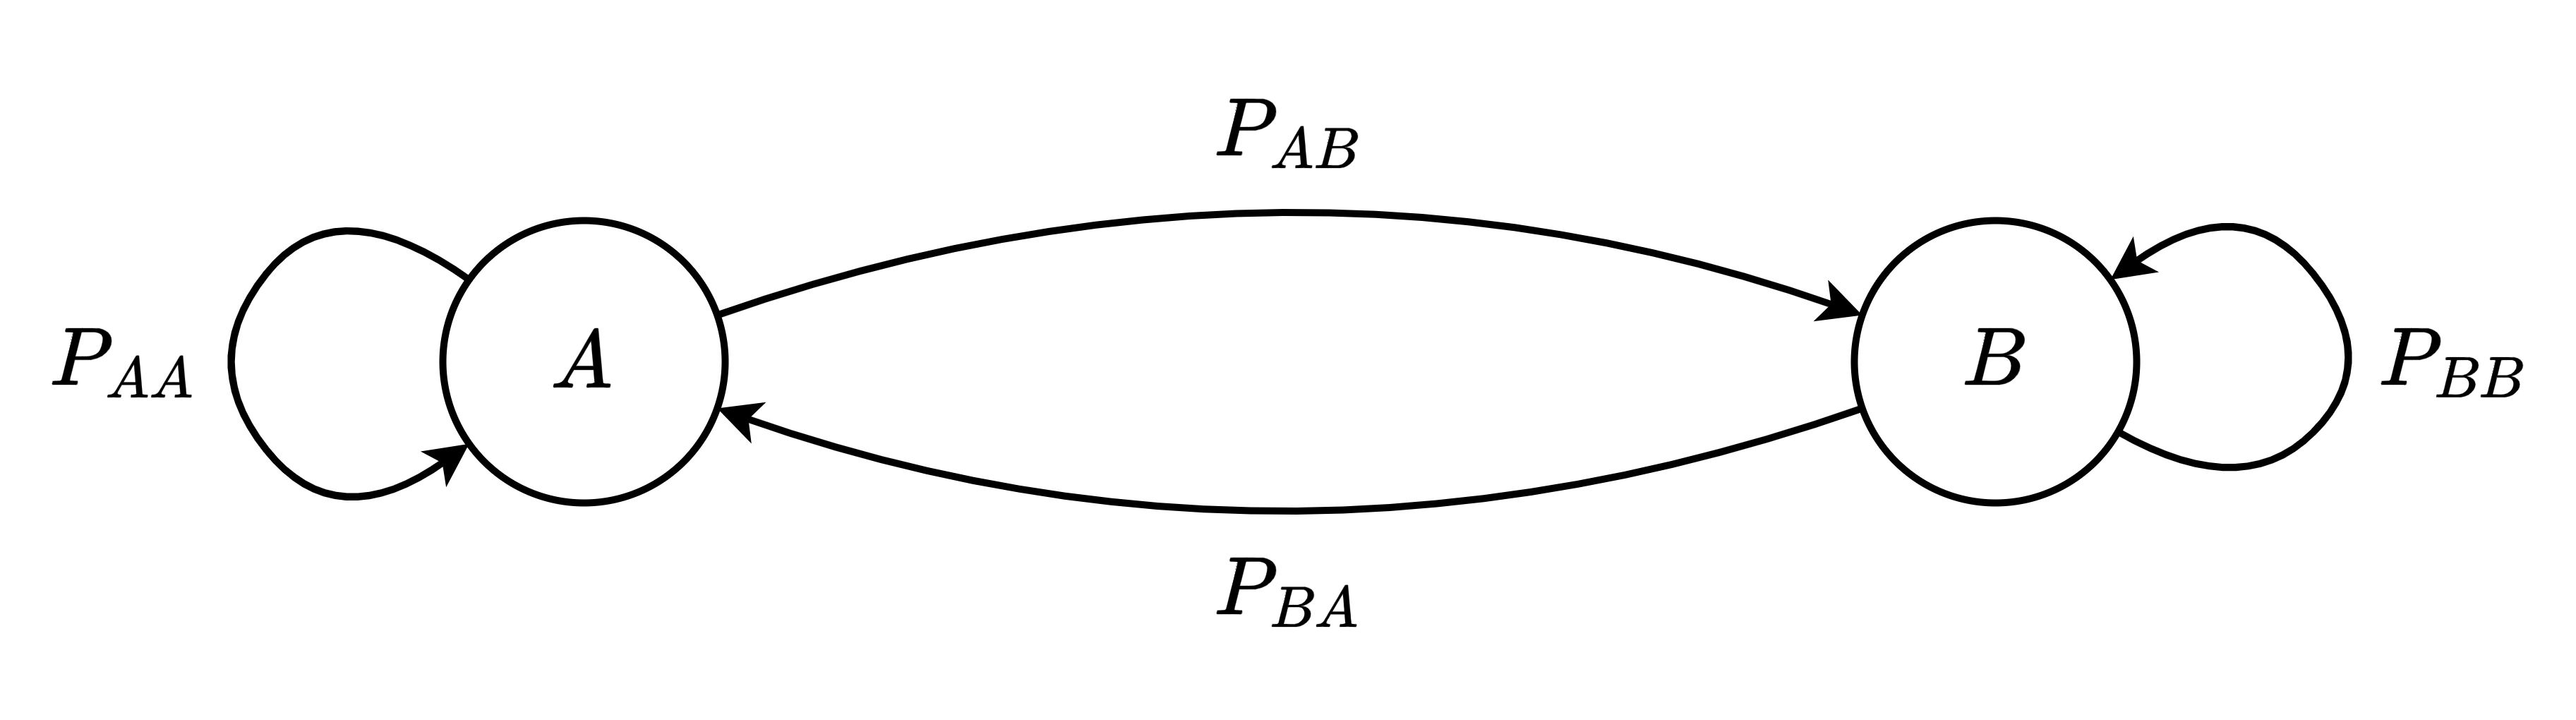
\includegraphics[width=0.8\textwidth]{diagram/DTE.png}
\end{center}
\subsection{Probabilidad de transici\'on en una etapa}
\begin{itemize}
    \item $P_{ij}$ : Probabilidad de pasar del estado i al estado j.
    Notar que:
    \begin{equation*}
        \sum_{j=1}^{n}{P_{ij}} = 1, \quad \forall i
    \end{equation*}

    \textbf{OBS:} En otras palabras la suma de las probabilidades de transici\'on de un estado a todos los dem\'as estados es igual a 1.
\end{itemize}
\subsection{Matriz de transici\'on}
Esta probabilidad se puede escribir en una matriz P de transici\'on en una etapa.
\begin{align*}
    P &= \left(\begin{matrix}
        P_{AA} & P_{AB} \\
        P_{BA} & P_{BB}
    \end{matrix} \right)
\end{align*}
\textbf{Supuesto 2:}
Las $P_{ij}$ no dependen de cuantas veces se transite de $i$ a $j$.

\newpage
\subsection{Ejemplo 1:}
En cierta localidad el clima puede estar Nublado (F), Lluvioso (R) y Soleado (S). \newline
Es decir en cada día existe un estado posible de entre F, R y S. \newline
Una realizaci\'on de este proceso es: $N\; N\; S\; S\; S\; R\; R\; N\; N\; ...$ \newline
En términos matemáticos, el proceso estocástico es:
\begin{align*}
    X_n &: \text{estado del clima en etapa(D\'ia)} \quad n \\
    \Omega &: \left\{N:\text{nublado}, S:\text{soleado}, R:\text{lluvioso}\right\}    
\end{align*}
\subsubsection*{Diagrama de transici\'on entre estados}
\begin{center}
    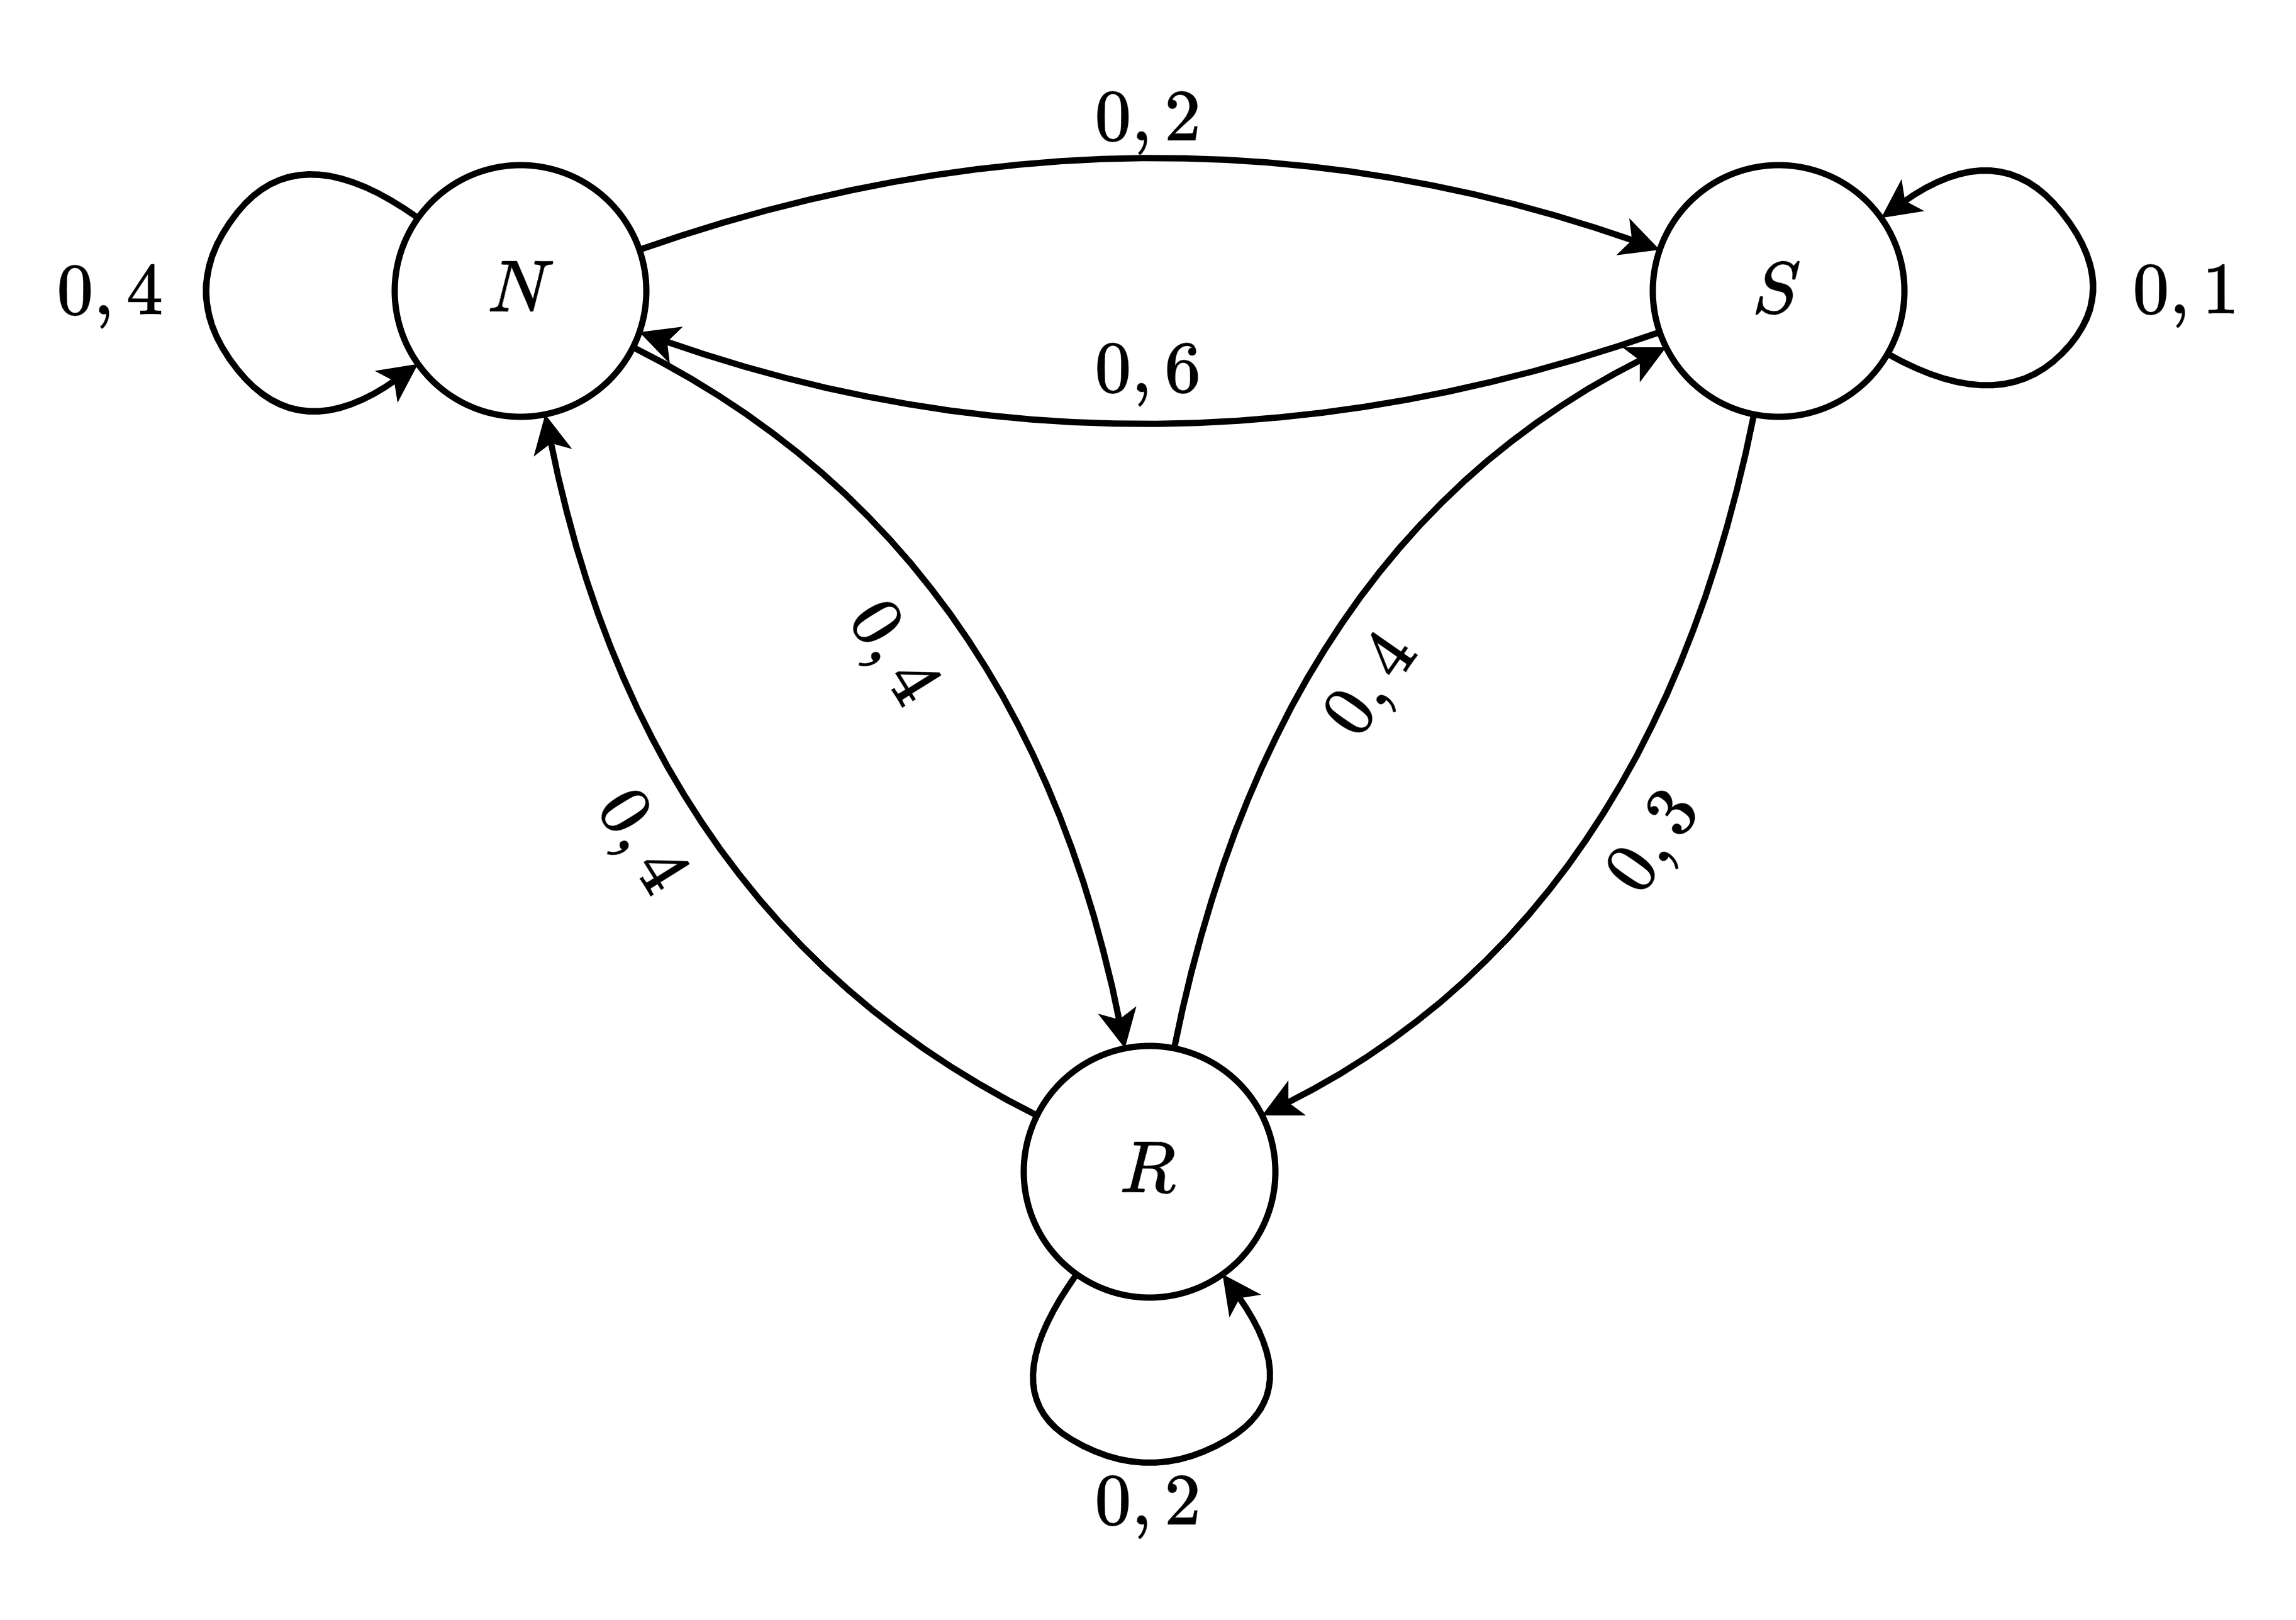
\includegraphics[width=0.8\textwidth]{diagram/DTE0.png}
\end{center}
\subsubsection*{Matriz de transici\'on}
\begin{align*}
    P &= \left(\begin{matrix}
        P_{NN} & P_{NS} & P_{NR} \\
        P_{SN} & P_{SS} & P_{SR} \\
        P_{RN} & P_{RS} & P_{RR}
    \end{matrix} \right) \\
    &= \left(\begin{matrix}
        0,4 & 0,2 & 0,4 \\
        0,6 & 0,1 & 0,3 \\
        0,4 & 0,4 & 0,2
    \end{matrix} \right)
\end{align*}

\textbf{OBS:} 
\begin{itemize}
    \item $P^n$ : es la matriz de transici\'on de probabilidades en $n$ etapas. 
    \begin{equation*}
        P^n = P \cdot P \cdot P \cdot ... \quad n \text{ veces}
    \end{equation*}

    \item $P_{ij}^{(n)}$ : Probabilidad de pasar del estado $i$ al estado $j$ en $n$ etapas.
    \begin{align*}
        P_{ij}^{(n)} &= (P^n)_{ij}
    \end{align*}
\end{itemize}
\newpage
\subsection{Problema 1:}
El ascensor de un edificio con bajo y dos pisos realiza viajes de uno a otro piso. El piso en el que finaliza el viaje n-\'esimo del ascensor sigue una cadena de Markov. Se sabe que la mitad de los viajes que parten del bajo se dirigen a cada uno de los otros dos pisos, mientras que si un viaje comienza en el primer piso, s\'olo el 25\% de las veces finaliza en el segundo. Por \'ultimo, si un trayecto comienza en el segundo piso, siempre finaliza en el bajo.
\begin{align*}
    X_n &: \text{Piso en que se encuentra ascensor en la etapa } \quad n \\
    \Omega &: \left\{0, 1, 2\right\}
\end{align*}
Si:
\begin{itemize}
    \item El proceso esta en el piso 0, puede ir a piso 1 o piso 2 con la misma probabilidad.
    \item El proceso esta en el piso 2 va a piso 0 directamente.
    \item El proceso esta en el piso 1 va a piso 0 el 25\% de las veces.
\end{itemize}
\begin{enumerate}
    \item Dibujar el diagrama de transici\'on entre estados.
    \begin{figure}[H]
        \centering
        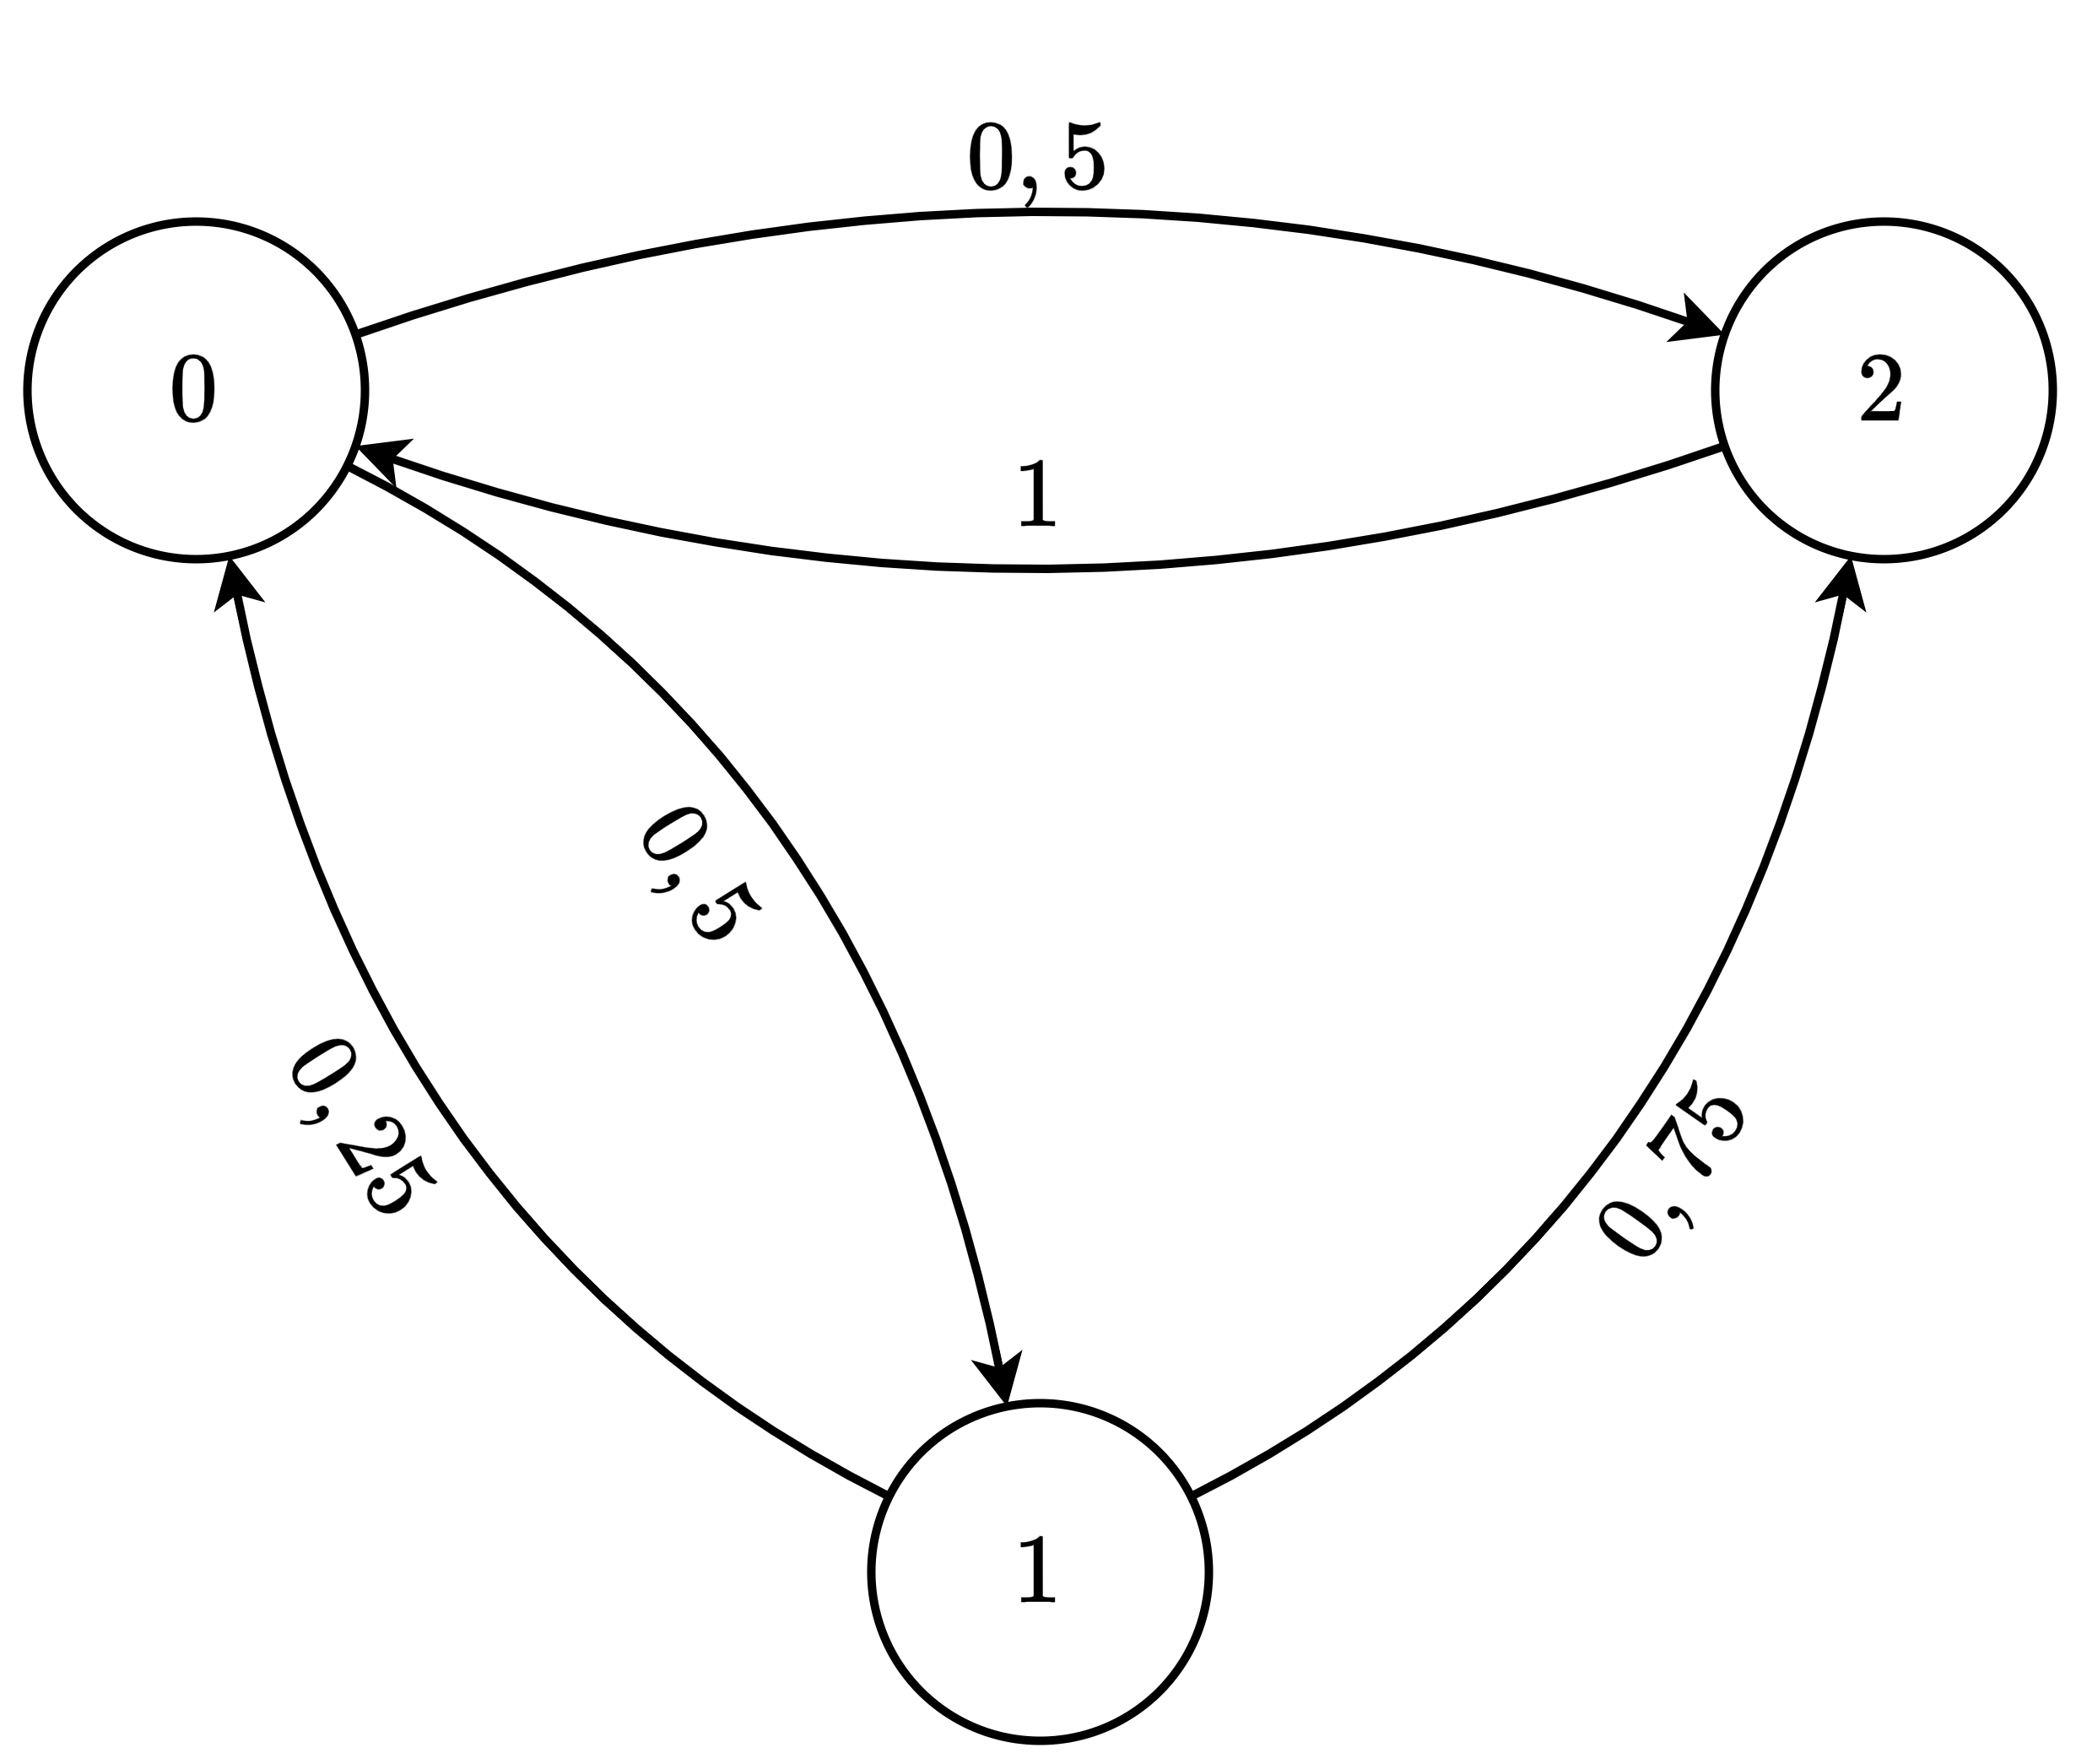
\includegraphics[width=0.5\textwidth]{diagram/DTE1.png}
    \end{figure}
    \item Encontrar la matriz P.
    \begin{align*}
        P &= \left(\begin{matrix}
            0 & 0,5 & 0,5 \\
            0,25 & 0 & 0,75 \\
            1 & 0 & 0
        \end{matrix} \right)
    \end{align*}

    \item Matriz de transici\'on en 2 etapas.
    \begin{align*}
        P^2 &= P \cdot P \\
        &= \left(\begin{matrix}
            0,625 & 0 & 0,375 \\
            0,75 & 0,125 & 0,125 \\
            0 & 0,5 & 0,5
        \end{matrix}\right)        
    \end{align*}
    \begin{equation*}
        P_{00}^{(2)} = 0 \cdot 0 + 0,5 \cdot 0,25 + 0,5 \cdot 1 = 0,625
    \end{equation*}
\end{enumerate}

\newpage
\subsection{Problema 2:}
En un juego participan dos jugadores, A y B. En cada turno, se lanza una moneda al aire. Si sale cara, A le debe \$1 a B. Si sale cruz, B le debe \$1 a A. Al principio, A tiene \$3 y B tiene \$2. El juego contin\'ua hasta que alguno de los dos se arruine. Calcular:
\newparagraph
\textbf{Matriz de transici\'on en una etapa}
\begin{center}
    \begin{tabular}{g|c|c|c|c|c|c|}
        \rowcolor{Celeste!50}
        \cellcolor{white} & \textbf{0} & \textbf{1} & \textbf{2} & \textbf{3} & \textbf{4} & \textbf{5} \\
        \hline
        \textbf{0} & 1 & 0 & 0 & 0 & 0 & 0 \\
        \hline
        \textbf{1} & 0,5 & 0 & 0,5 & 0 & 0 & 0 \\
        \hline
        \textbf{2} & 0 & 0,5 & 0 & 0,5 & 0 & 0 \\
        \hline
        \textbf{3} & 0 & 0 & 0,5 & 0 & 0,5 & 0 \\
        \hline
        \textbf{4} & 0 & 0 & 0 & 0,5 & 0 & 0,5 \\
        \hline
        \textbf{5} & 0 & 0 & 0 & 0 & 0 & 1 \\
        \hline
    \end{tabular}
\end{center}
\textbf{Diagrama de transici\'on entre estados}
\begin{center}
    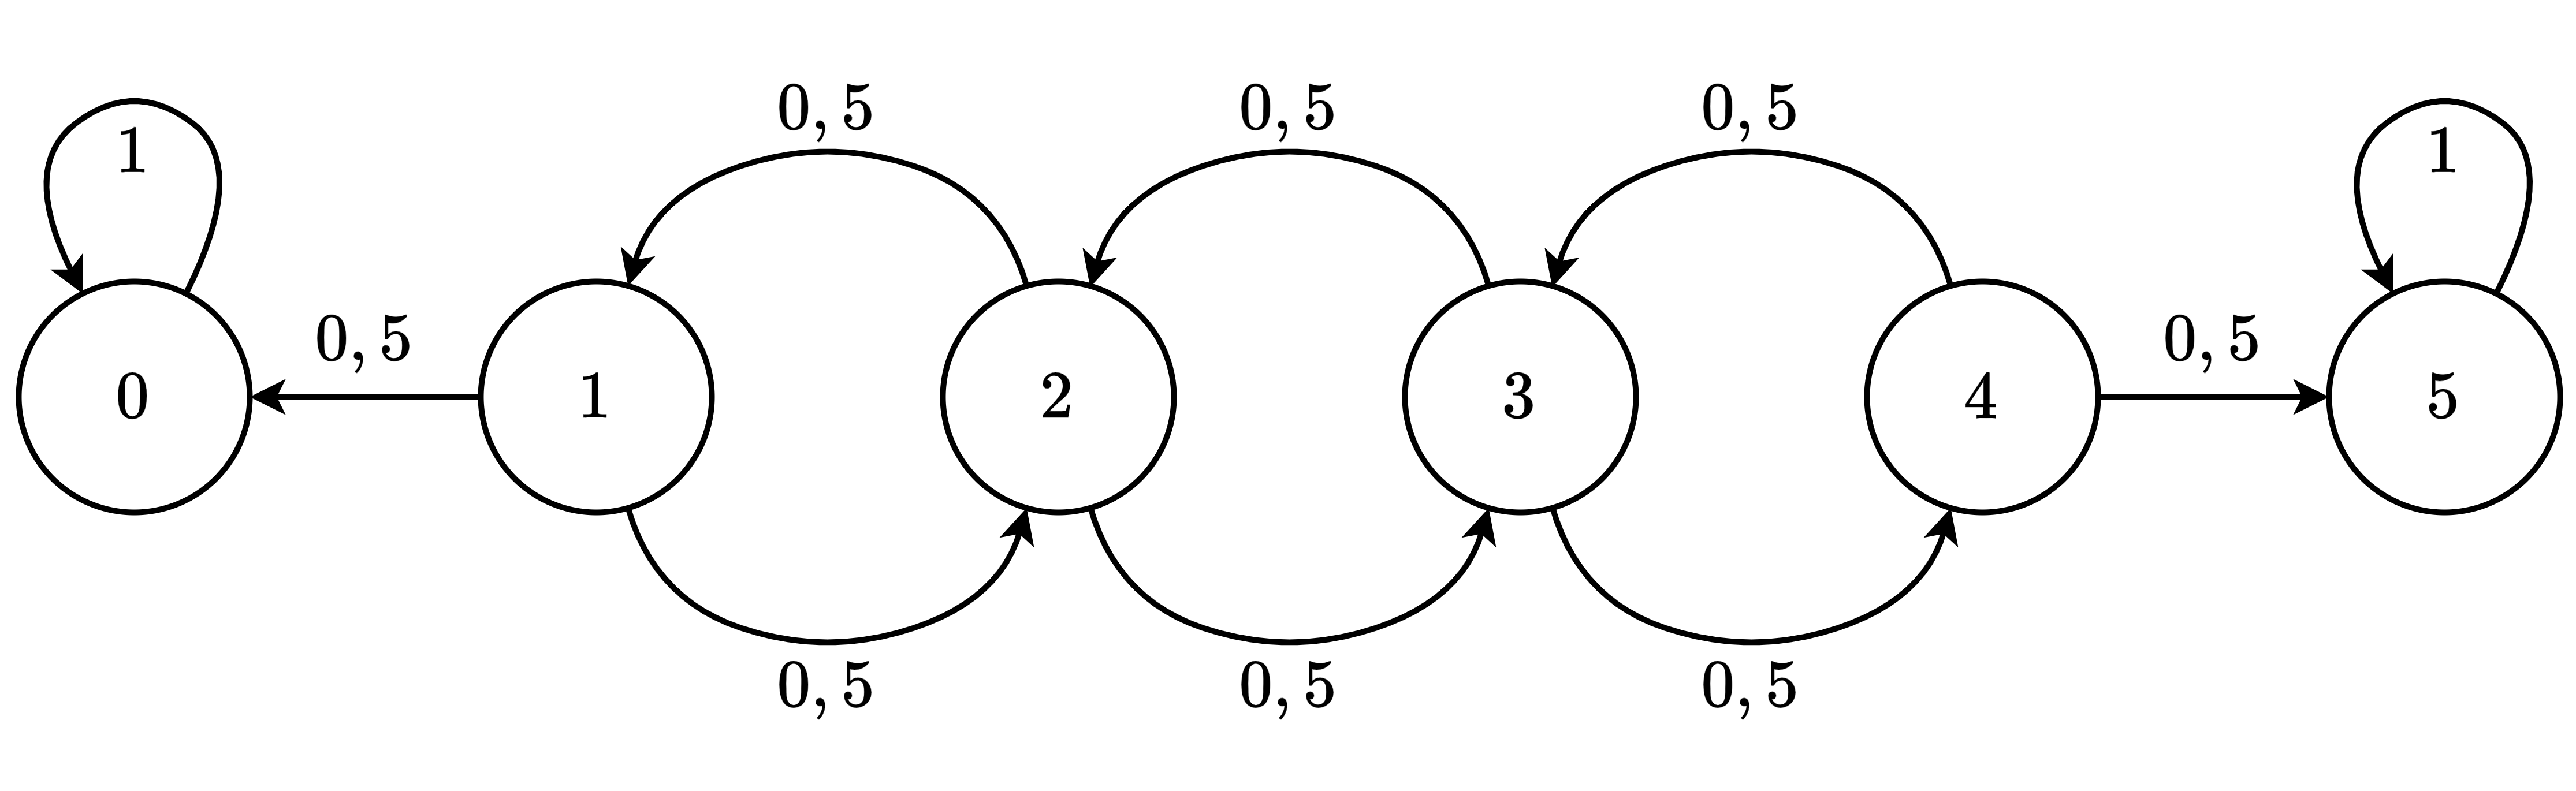
\includegraphics[width=0.9\textwidth]{diagram/DTE2.png}
\end{center}
\begin{enumerate}
    \item La probabilidad de que A termine arruin\'andose.
    \item La probabilidad de que B termine arruin\'andose.
    \item El n\'umero medio de tiradas que tarda en acabar el juego.
\end{enumerate}

\newpage
\subsection{Problema 3:}
Se lanza un dado repetidas veces. Cada vez que sale menor que 5 se pierde \$1, y cada vez que sale 5 o 6 se gana \$1. El juego acaba cuando se tiene \$0 o \$100.
\begin{itemize}
    \item Sea $X_t$ : Estado de cuentas en el instante t. Tenemos que ${X_t}$ es una CM.
    \item S = \{0, 1, 2, ..., 100\}
\end{itemize}
\begin{enumerate}
    \item Dibujar el diagrama de transici\'on entre estados.
    \begin{figure}[H]
        \centering
        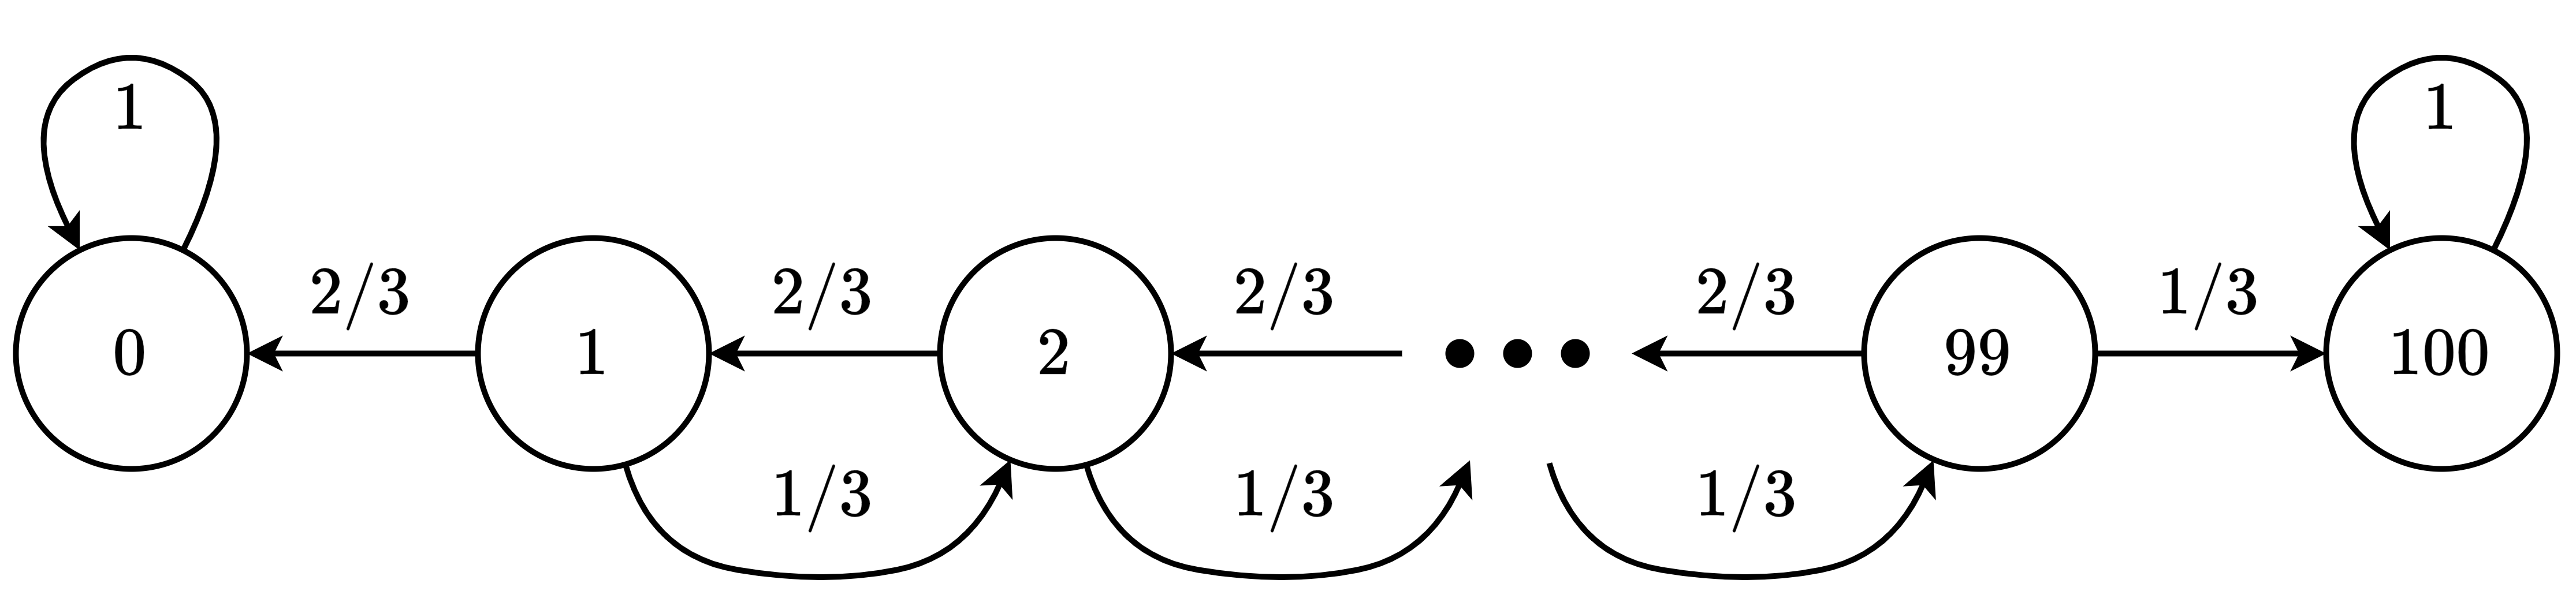
\includegraphics[width=0.9\textwidth]{diagram/DTE3.png}
    \end{figure}
\end{enumerate}

\newpage
\subsection{Clasificaci\'on de estados}
\begin{center}
    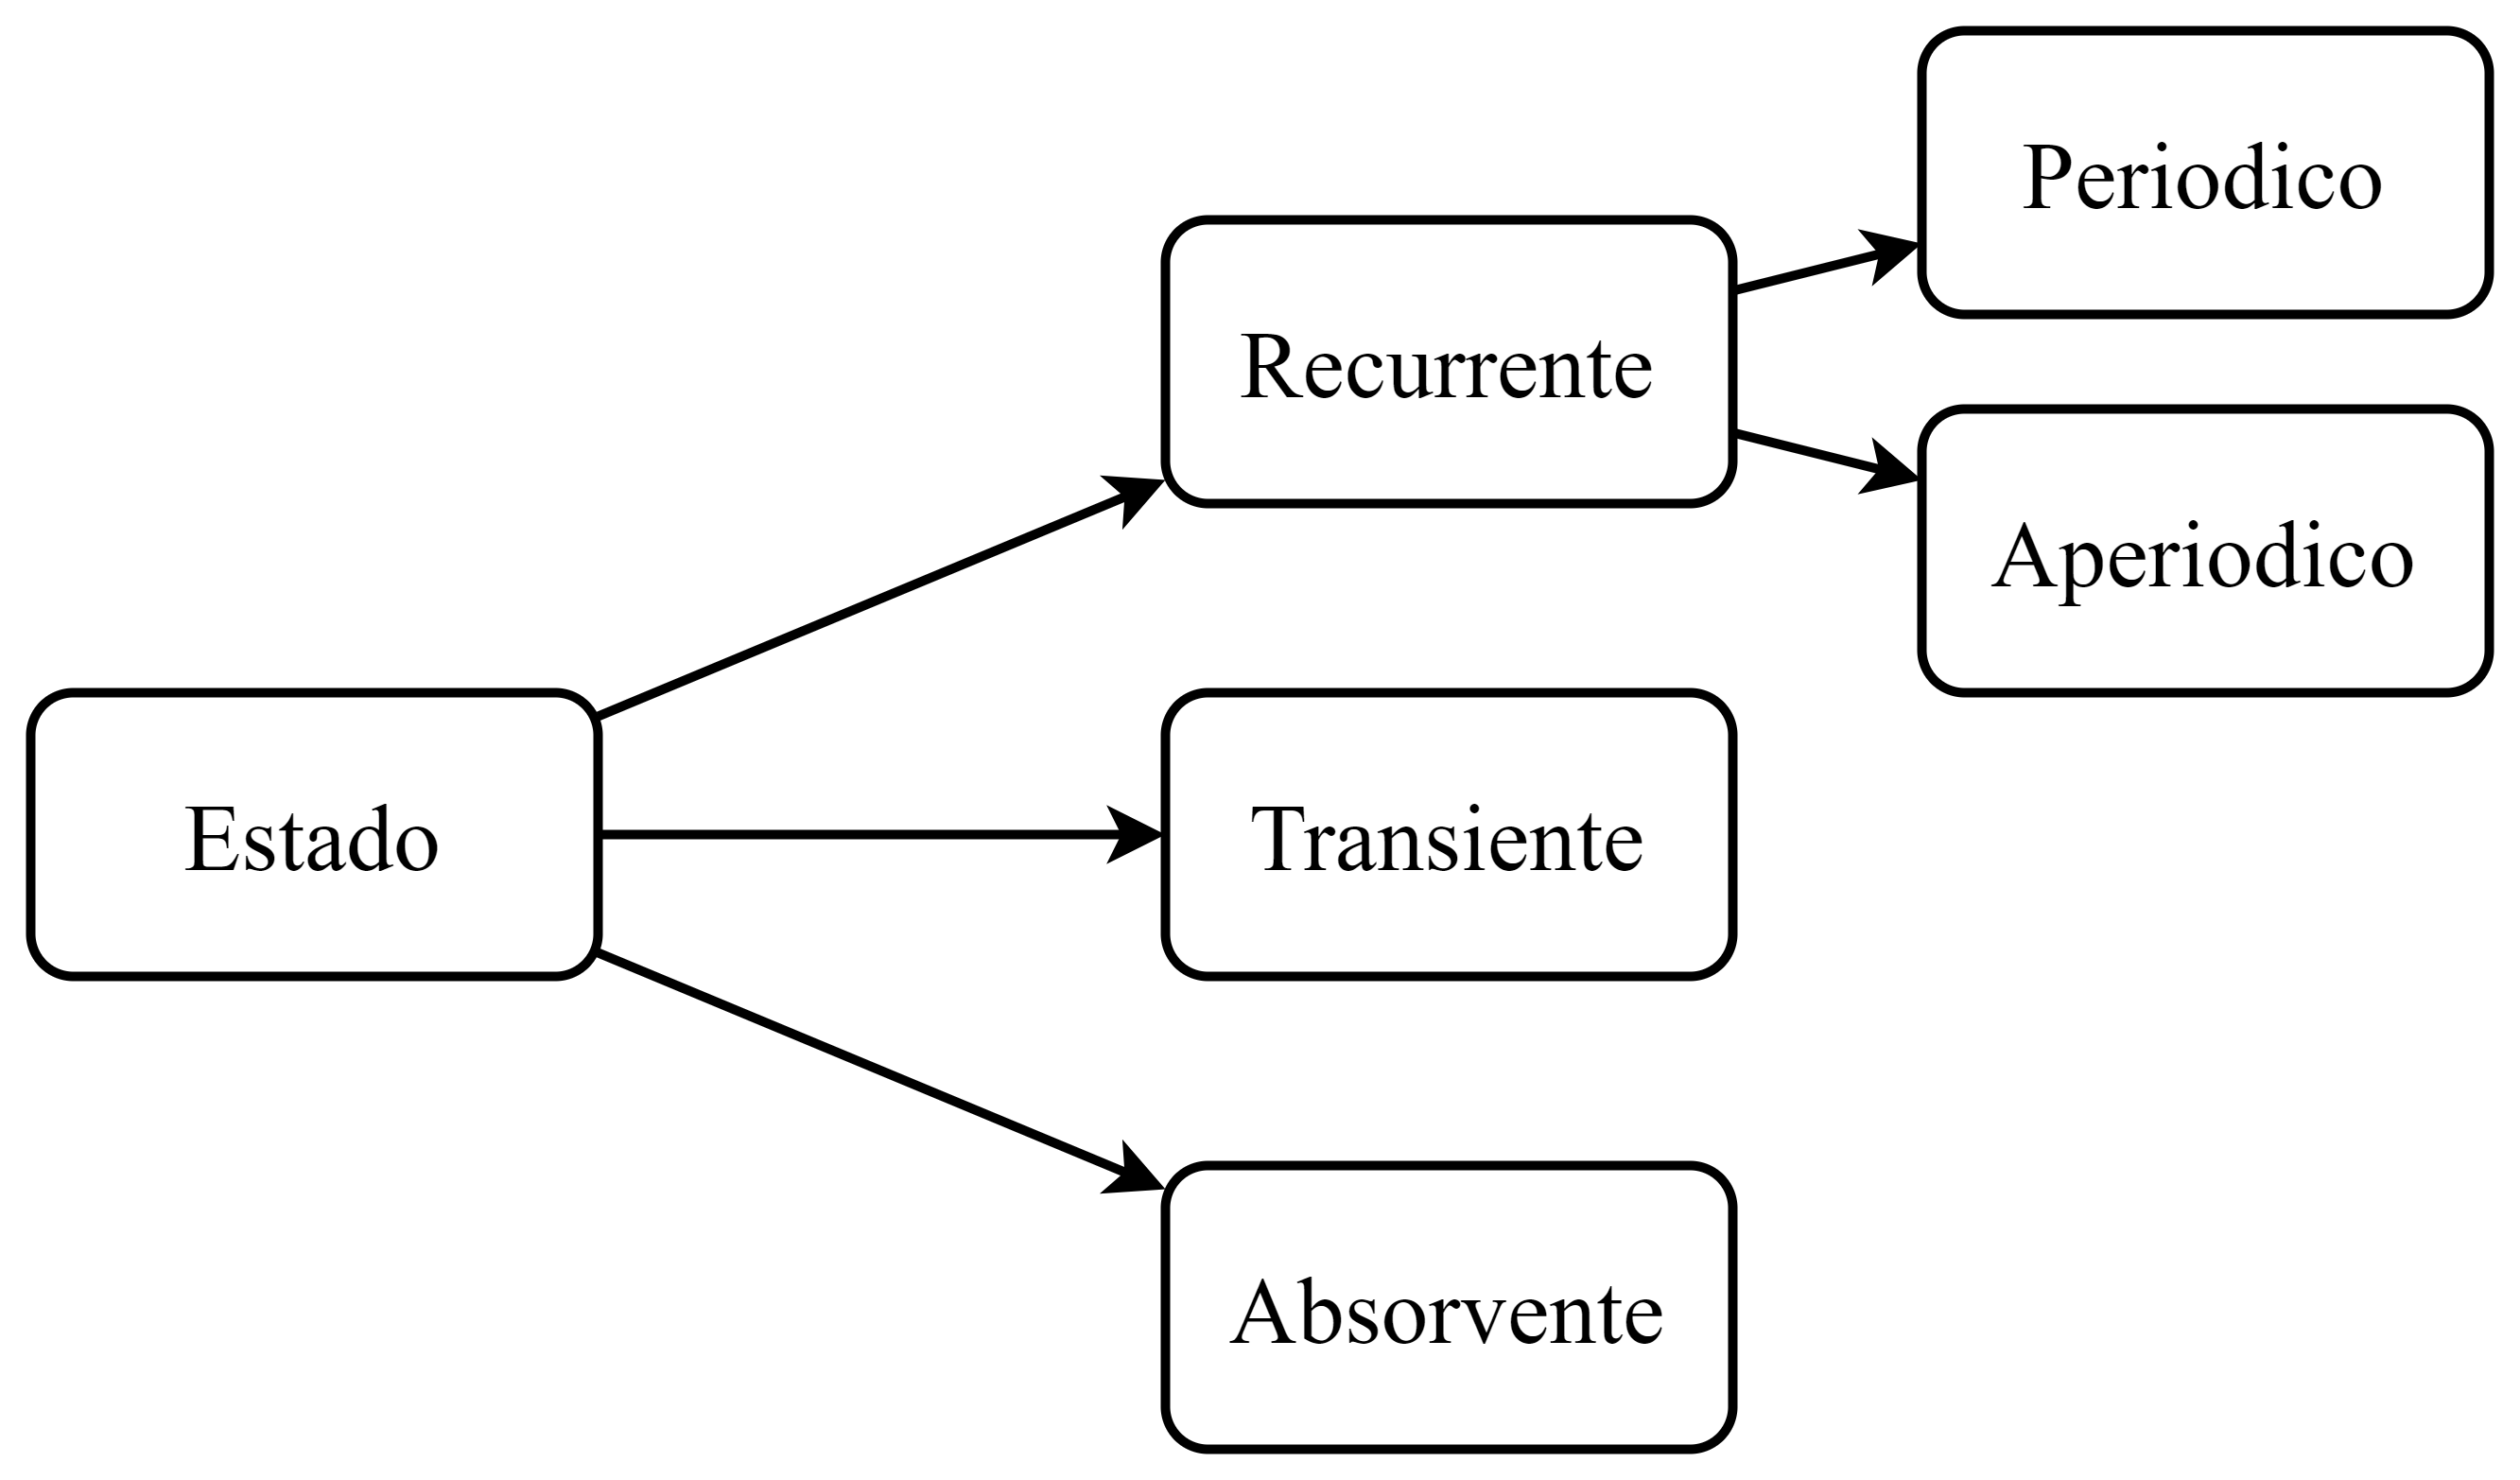
\includegraphics[width=0.7\textwidth]{diagram/ClasificacionEstados.png}
\end{center}
\begin{itemize}
    \item Diremos que 2 estados son \textbf{comunicantes}, si:
    \begin{equation*}
        i \rightarrow j \quad \wedge \quad j \rightarrow i
    \end{equation*}

    \item Los estados que se comunican entre si son de una misma clase $C_i$ y todos son del mismo tipo.
    
    \item La relaci\'on $i \leftrightarrow j$ es transitiva, es decir:
    \begin{equation*}
        i \leftrightarrow j \quad \wedge \quad j \leftrightarrow k \quad \Rightarrow \quad i \leftrightarrow k
    \end{equation*}
\end{itemize}
\subsubsection{Recurrentes}
Cuando la cadena puede visitar dicho estado un numero \textbf{INFINITO} de veces.
\begin{itemize}
    \item Aperiodico.
    \begin{center}
        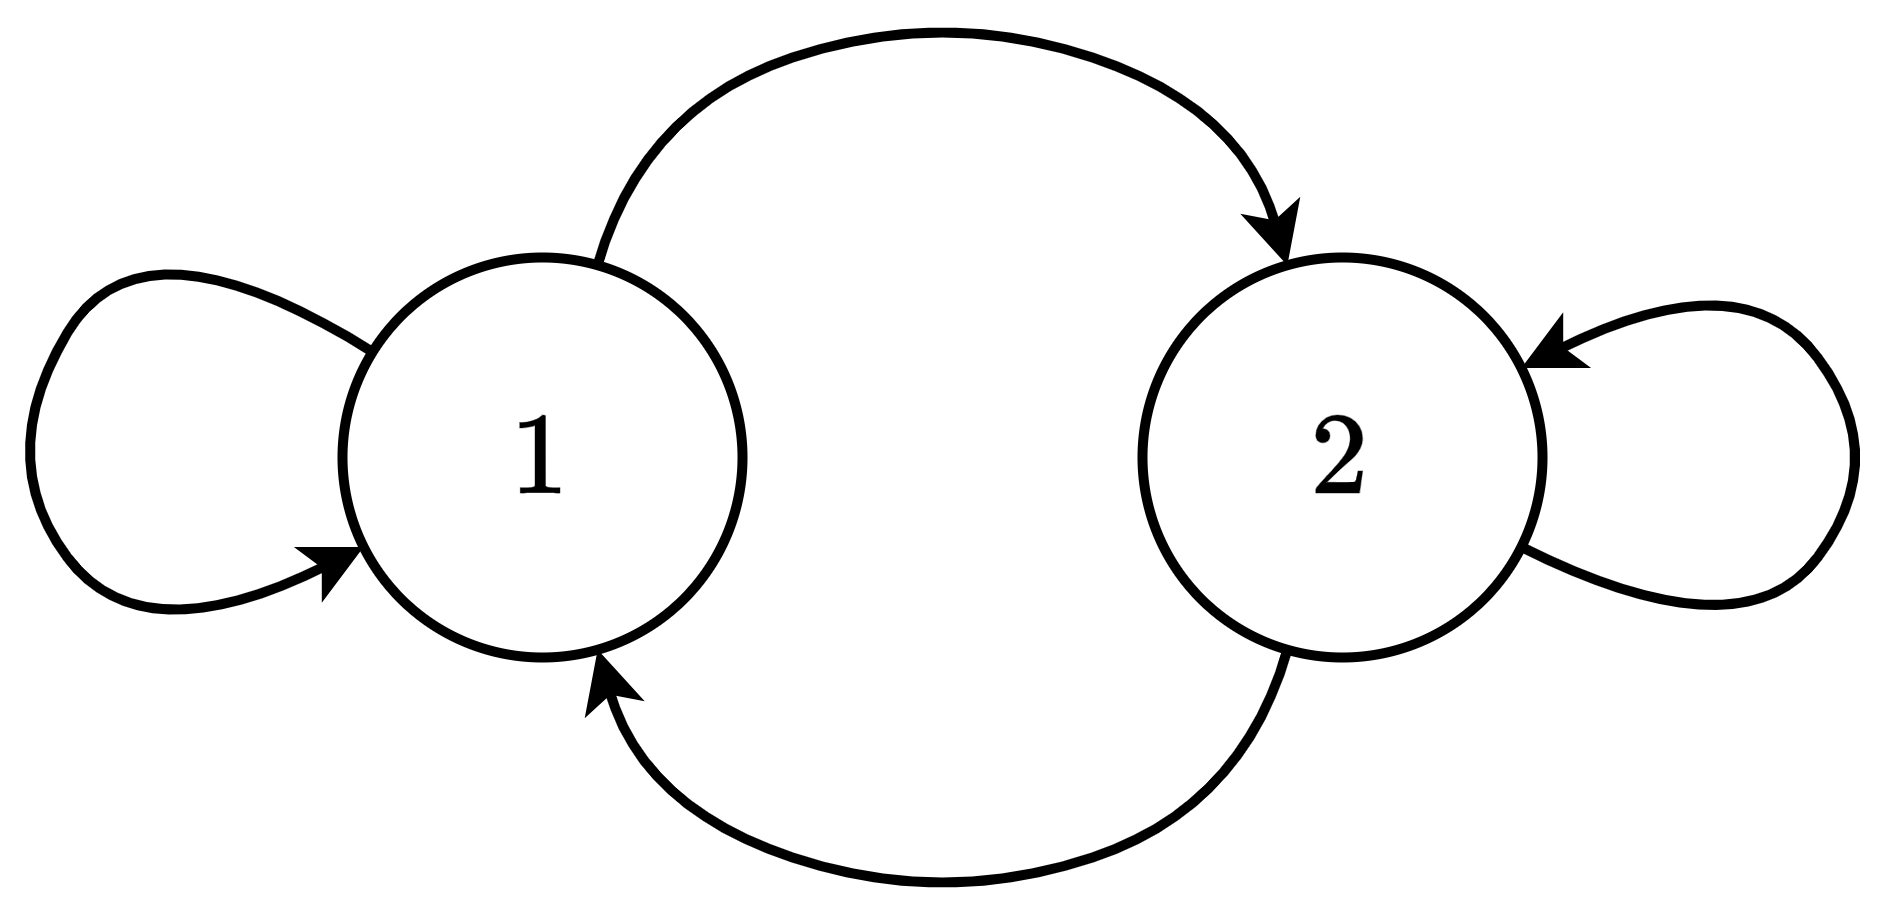
\includegraphics[width=0.4\textwidth]{diagram/Aperiodico.png}
    \end{center}

    \item Periodico.
    \begin{center}
        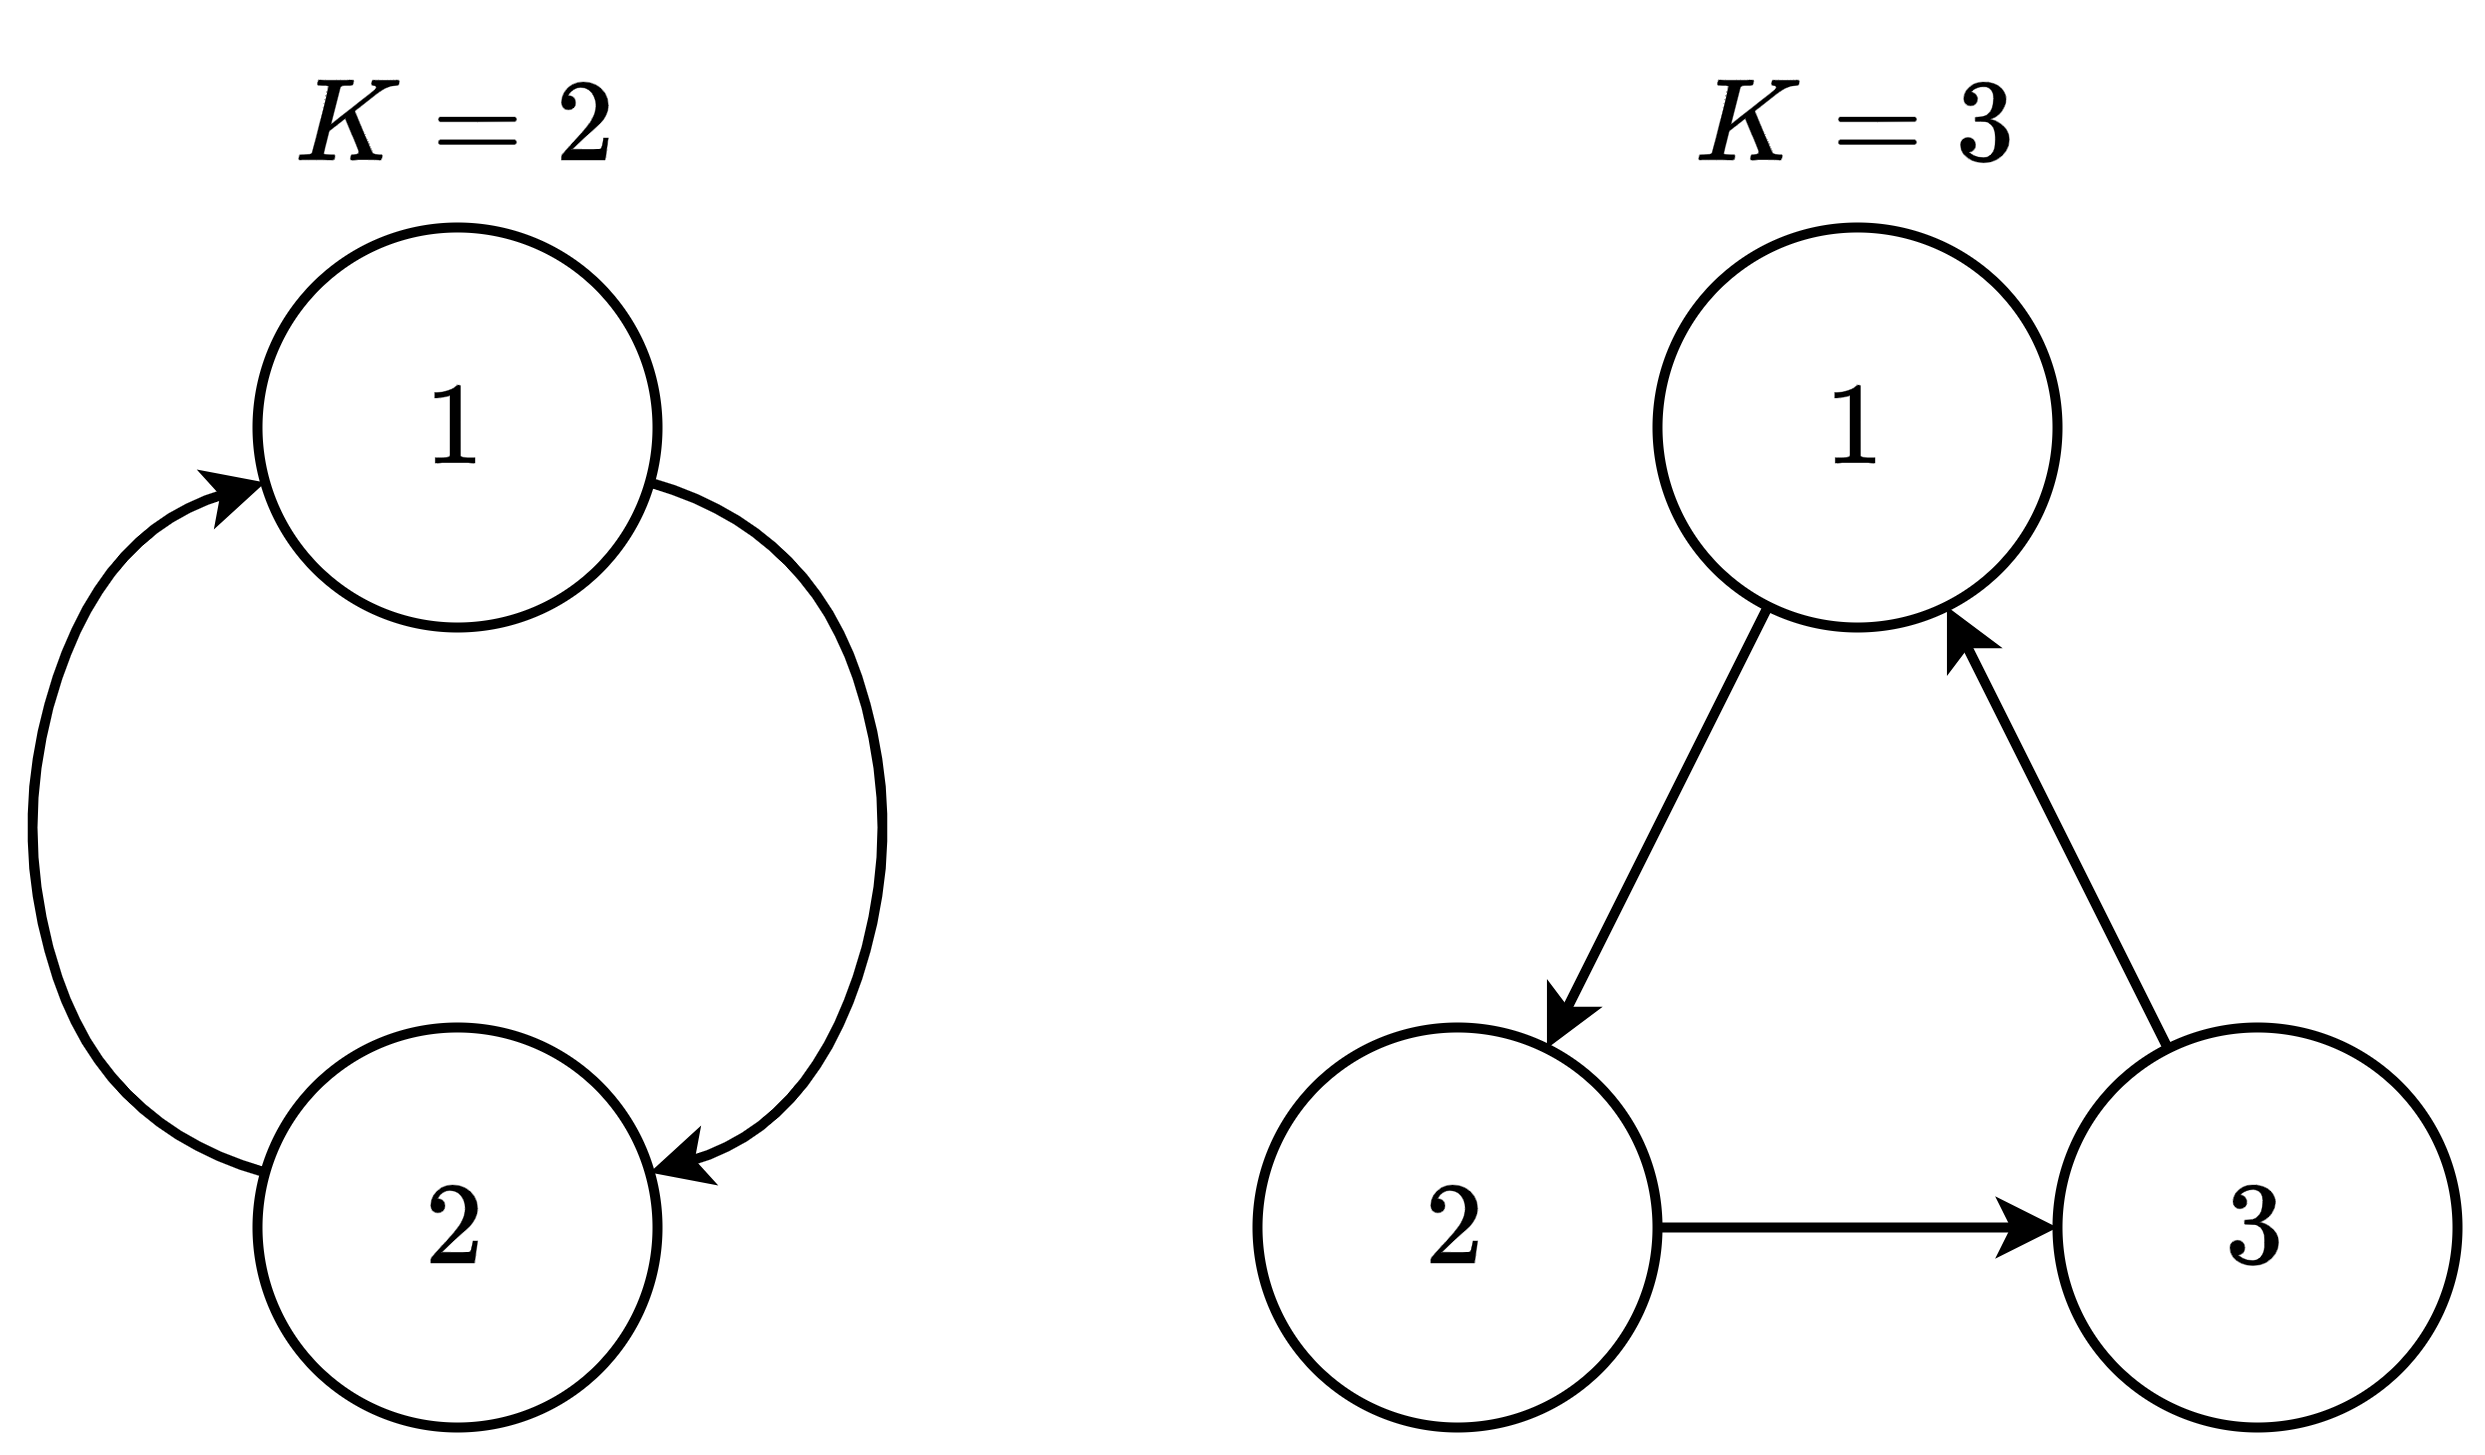
\includegraphics[width=0.5\textwidth]{diagram/Periodico.png}
    \end{center}
\end{itemize}

\subsubsection{Transientes}
Cuando la cadena puede visitar dicho estado solo un numero \textbf{FINITO} de veces.
\begin{center}
    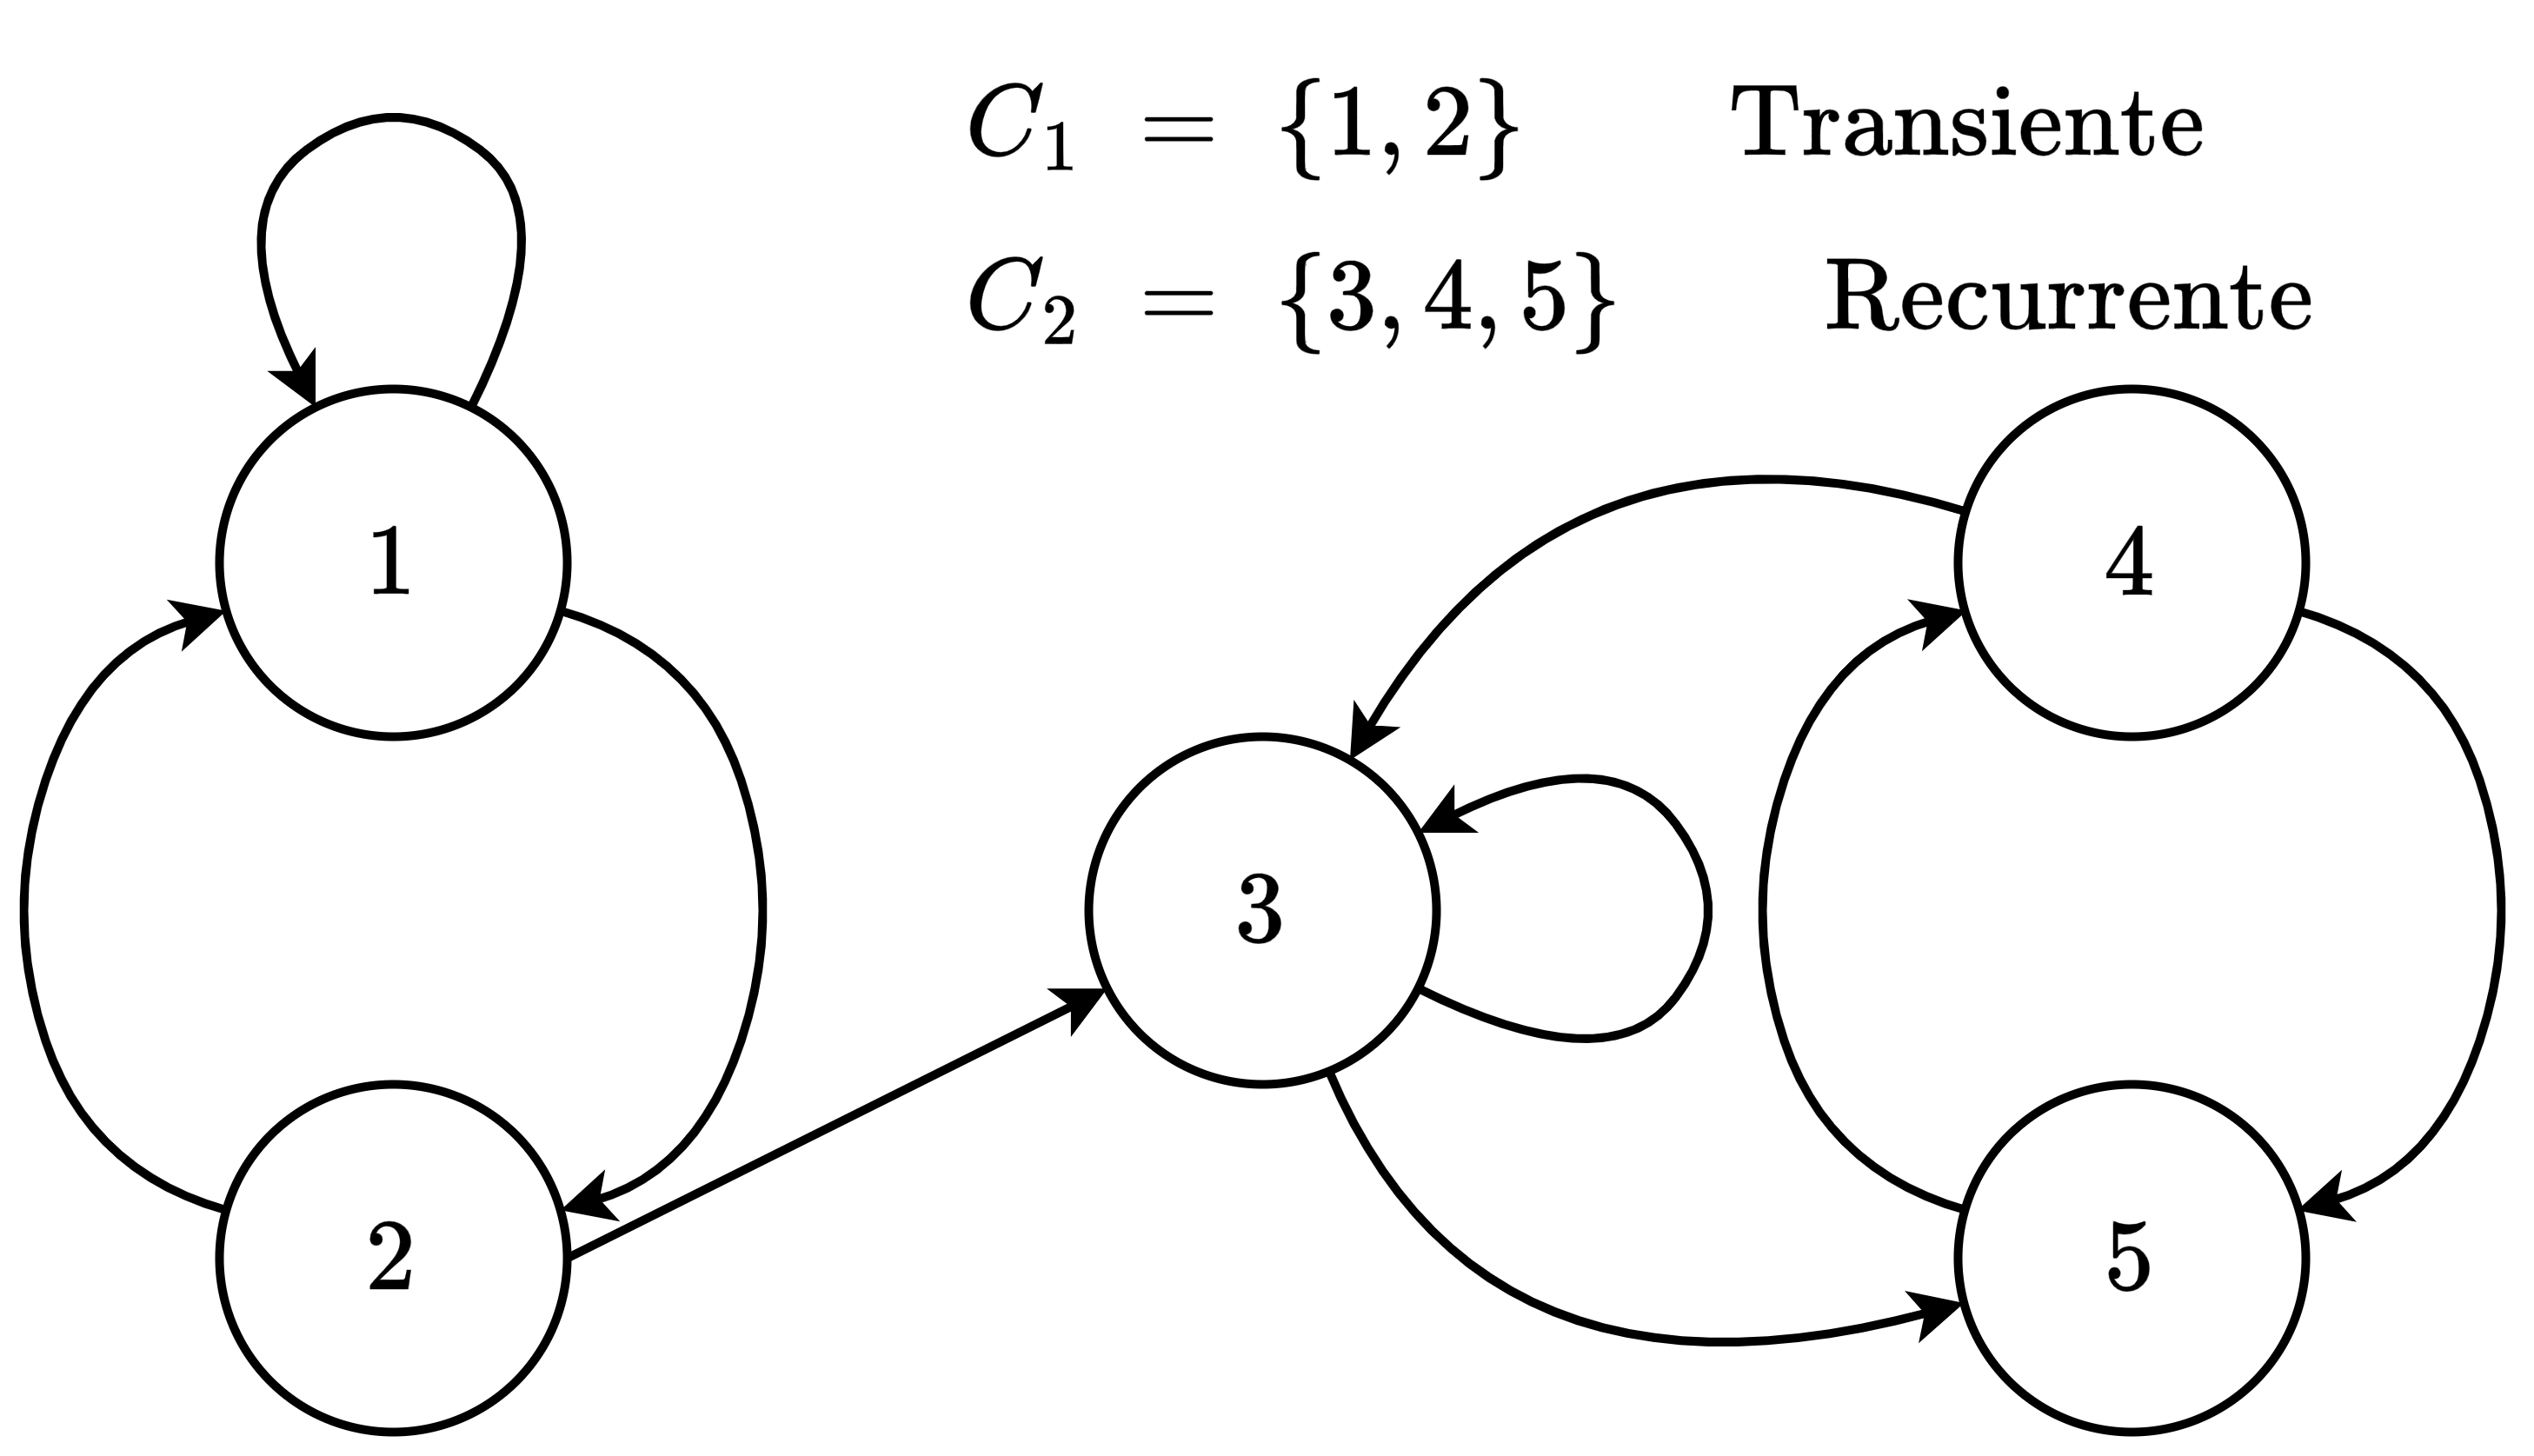
\includegraphics[width=0.7\textwidth]{diagram/Transiente.png}
\end{center}
\subsubsection{Absorvente}
\begin{center}
    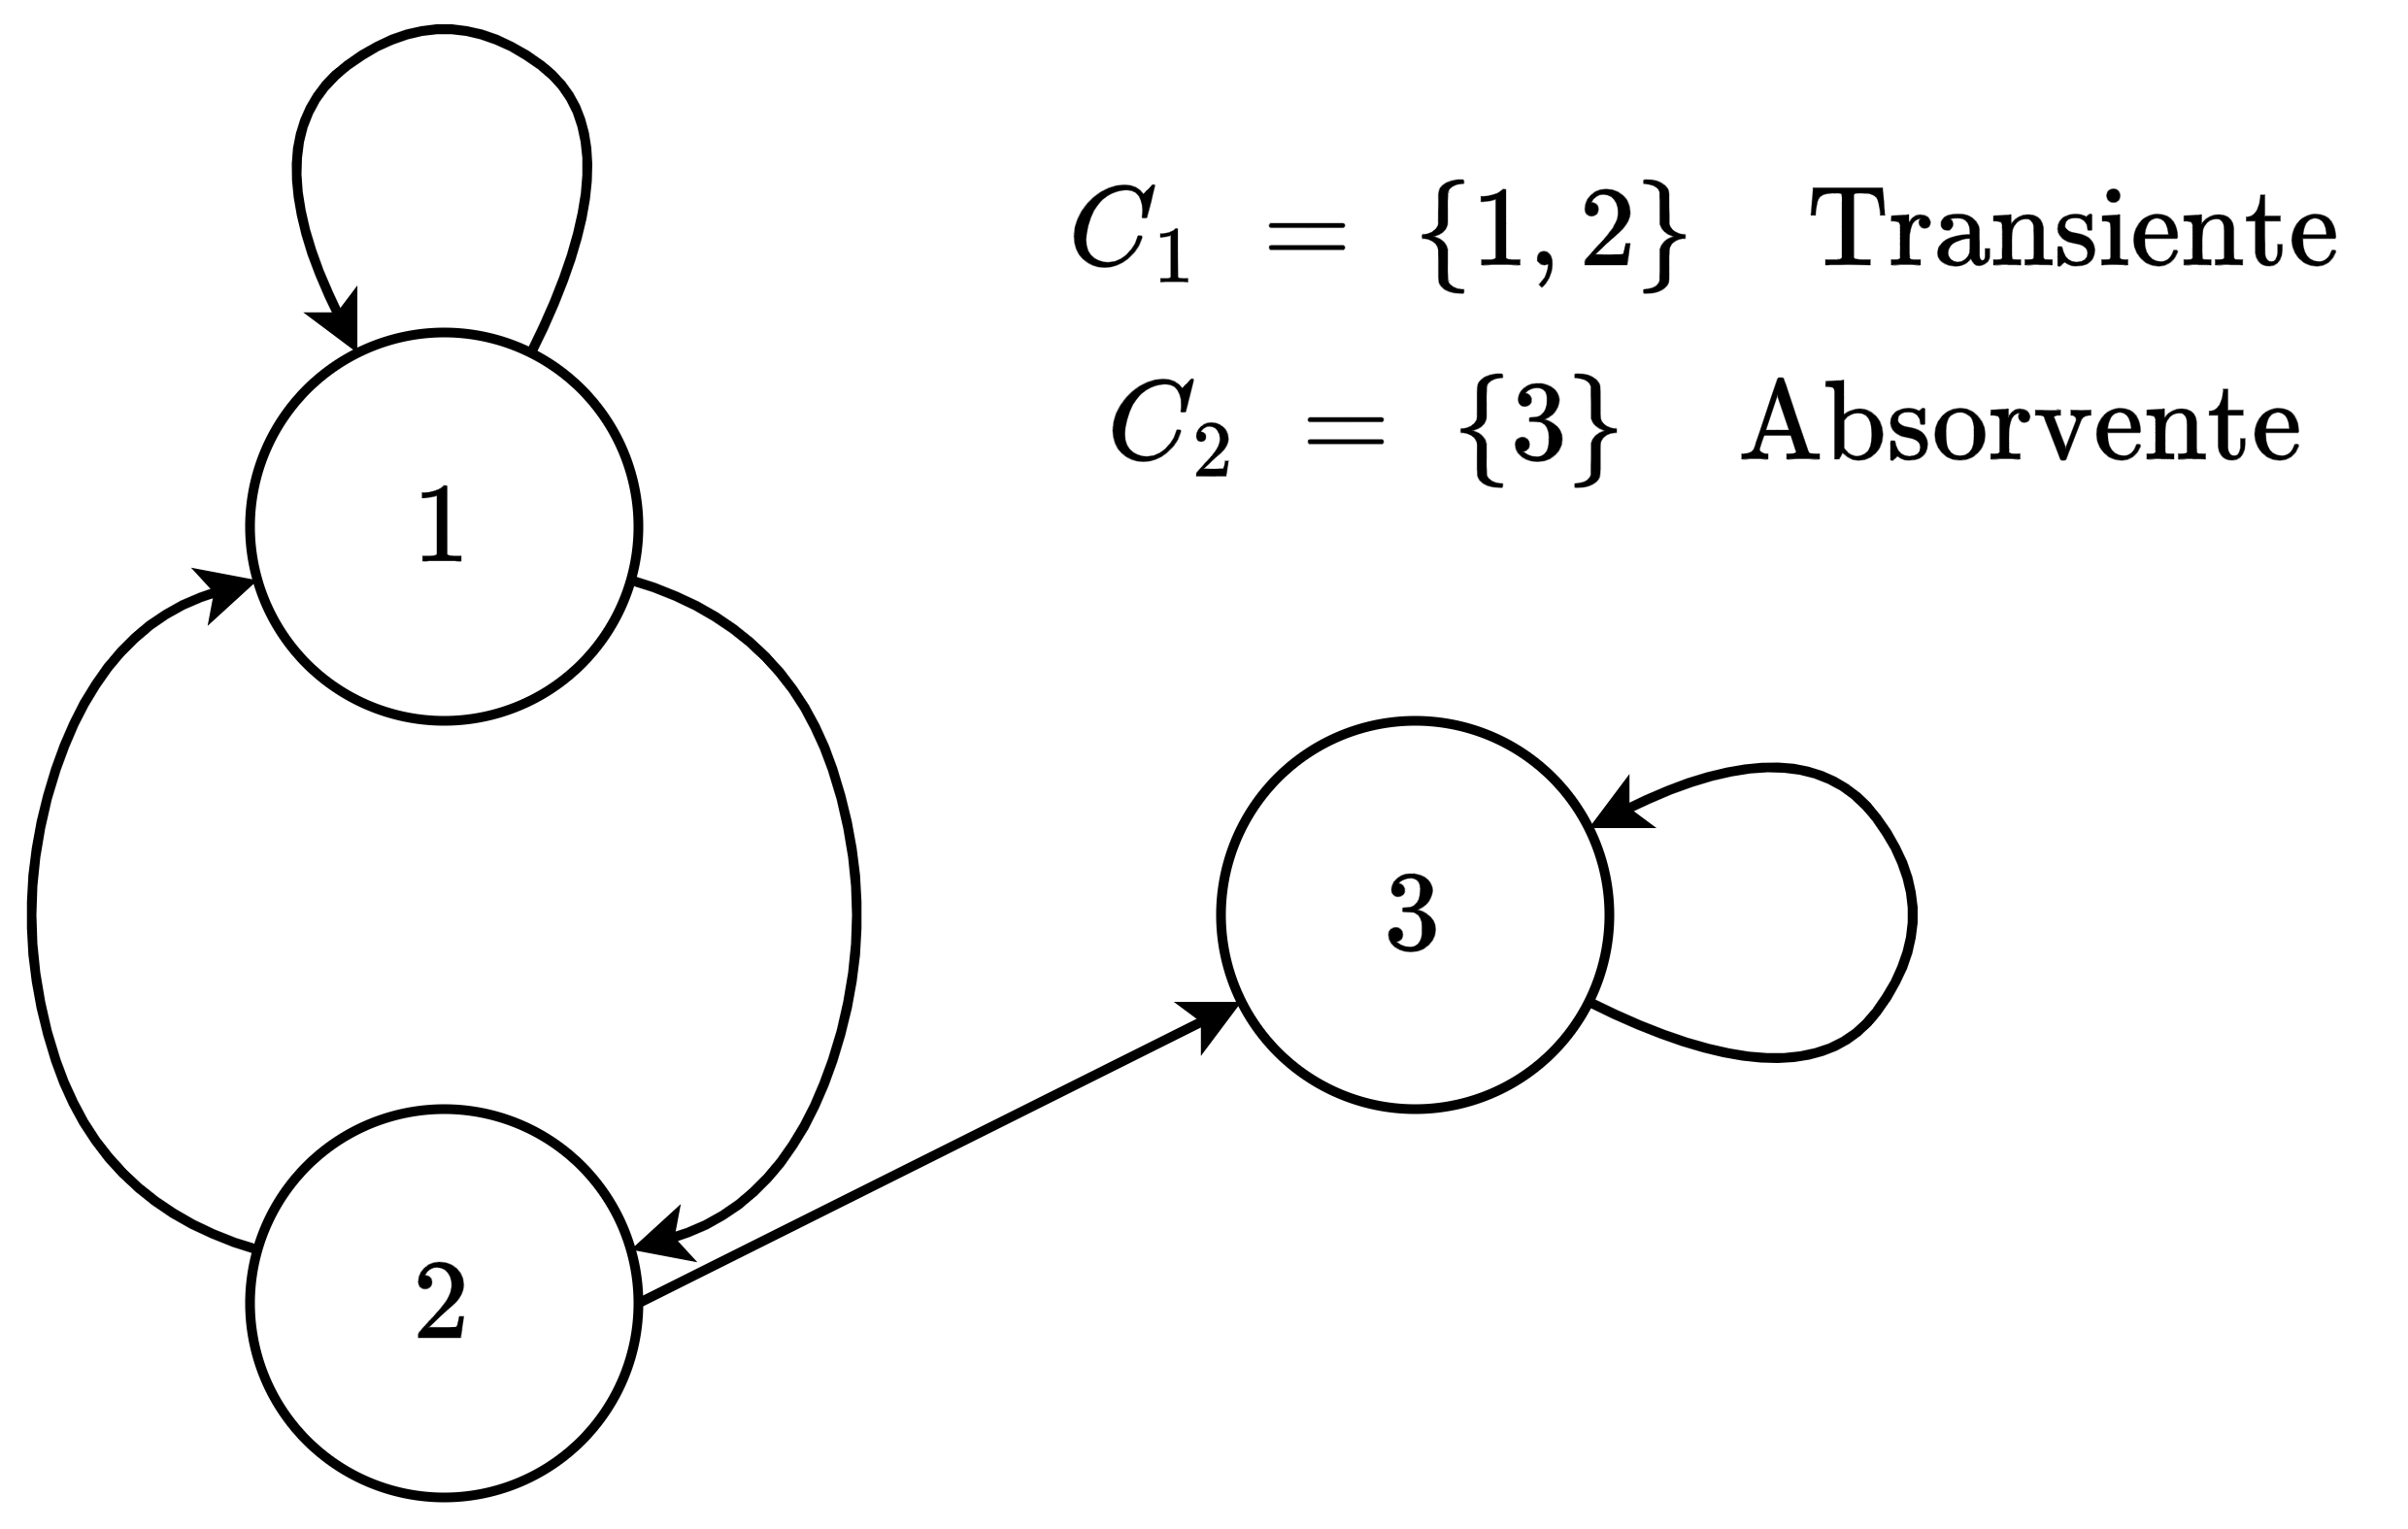
\includegraphics[width=0.6\textwidth]{diagram/Absorvente.png}
\end{center}

\newpage
\subsection{Clases de cadenas}
\subsubsection{Irreducible}
Una cadena se dice irreducible si sus estados forman una sola clase.
Puede ser:
\begin{itemize}
    \item Transiente.
    \item Recurrente aperi\'odica.
    \item Recurrente peri\'odica.
\end{itemize}
\subsubsection{Reducible / Reductible}
Una cadena se dice reducible si sus estados forman m\'as de una clase.
\begin{figure}[H]
    \centering
    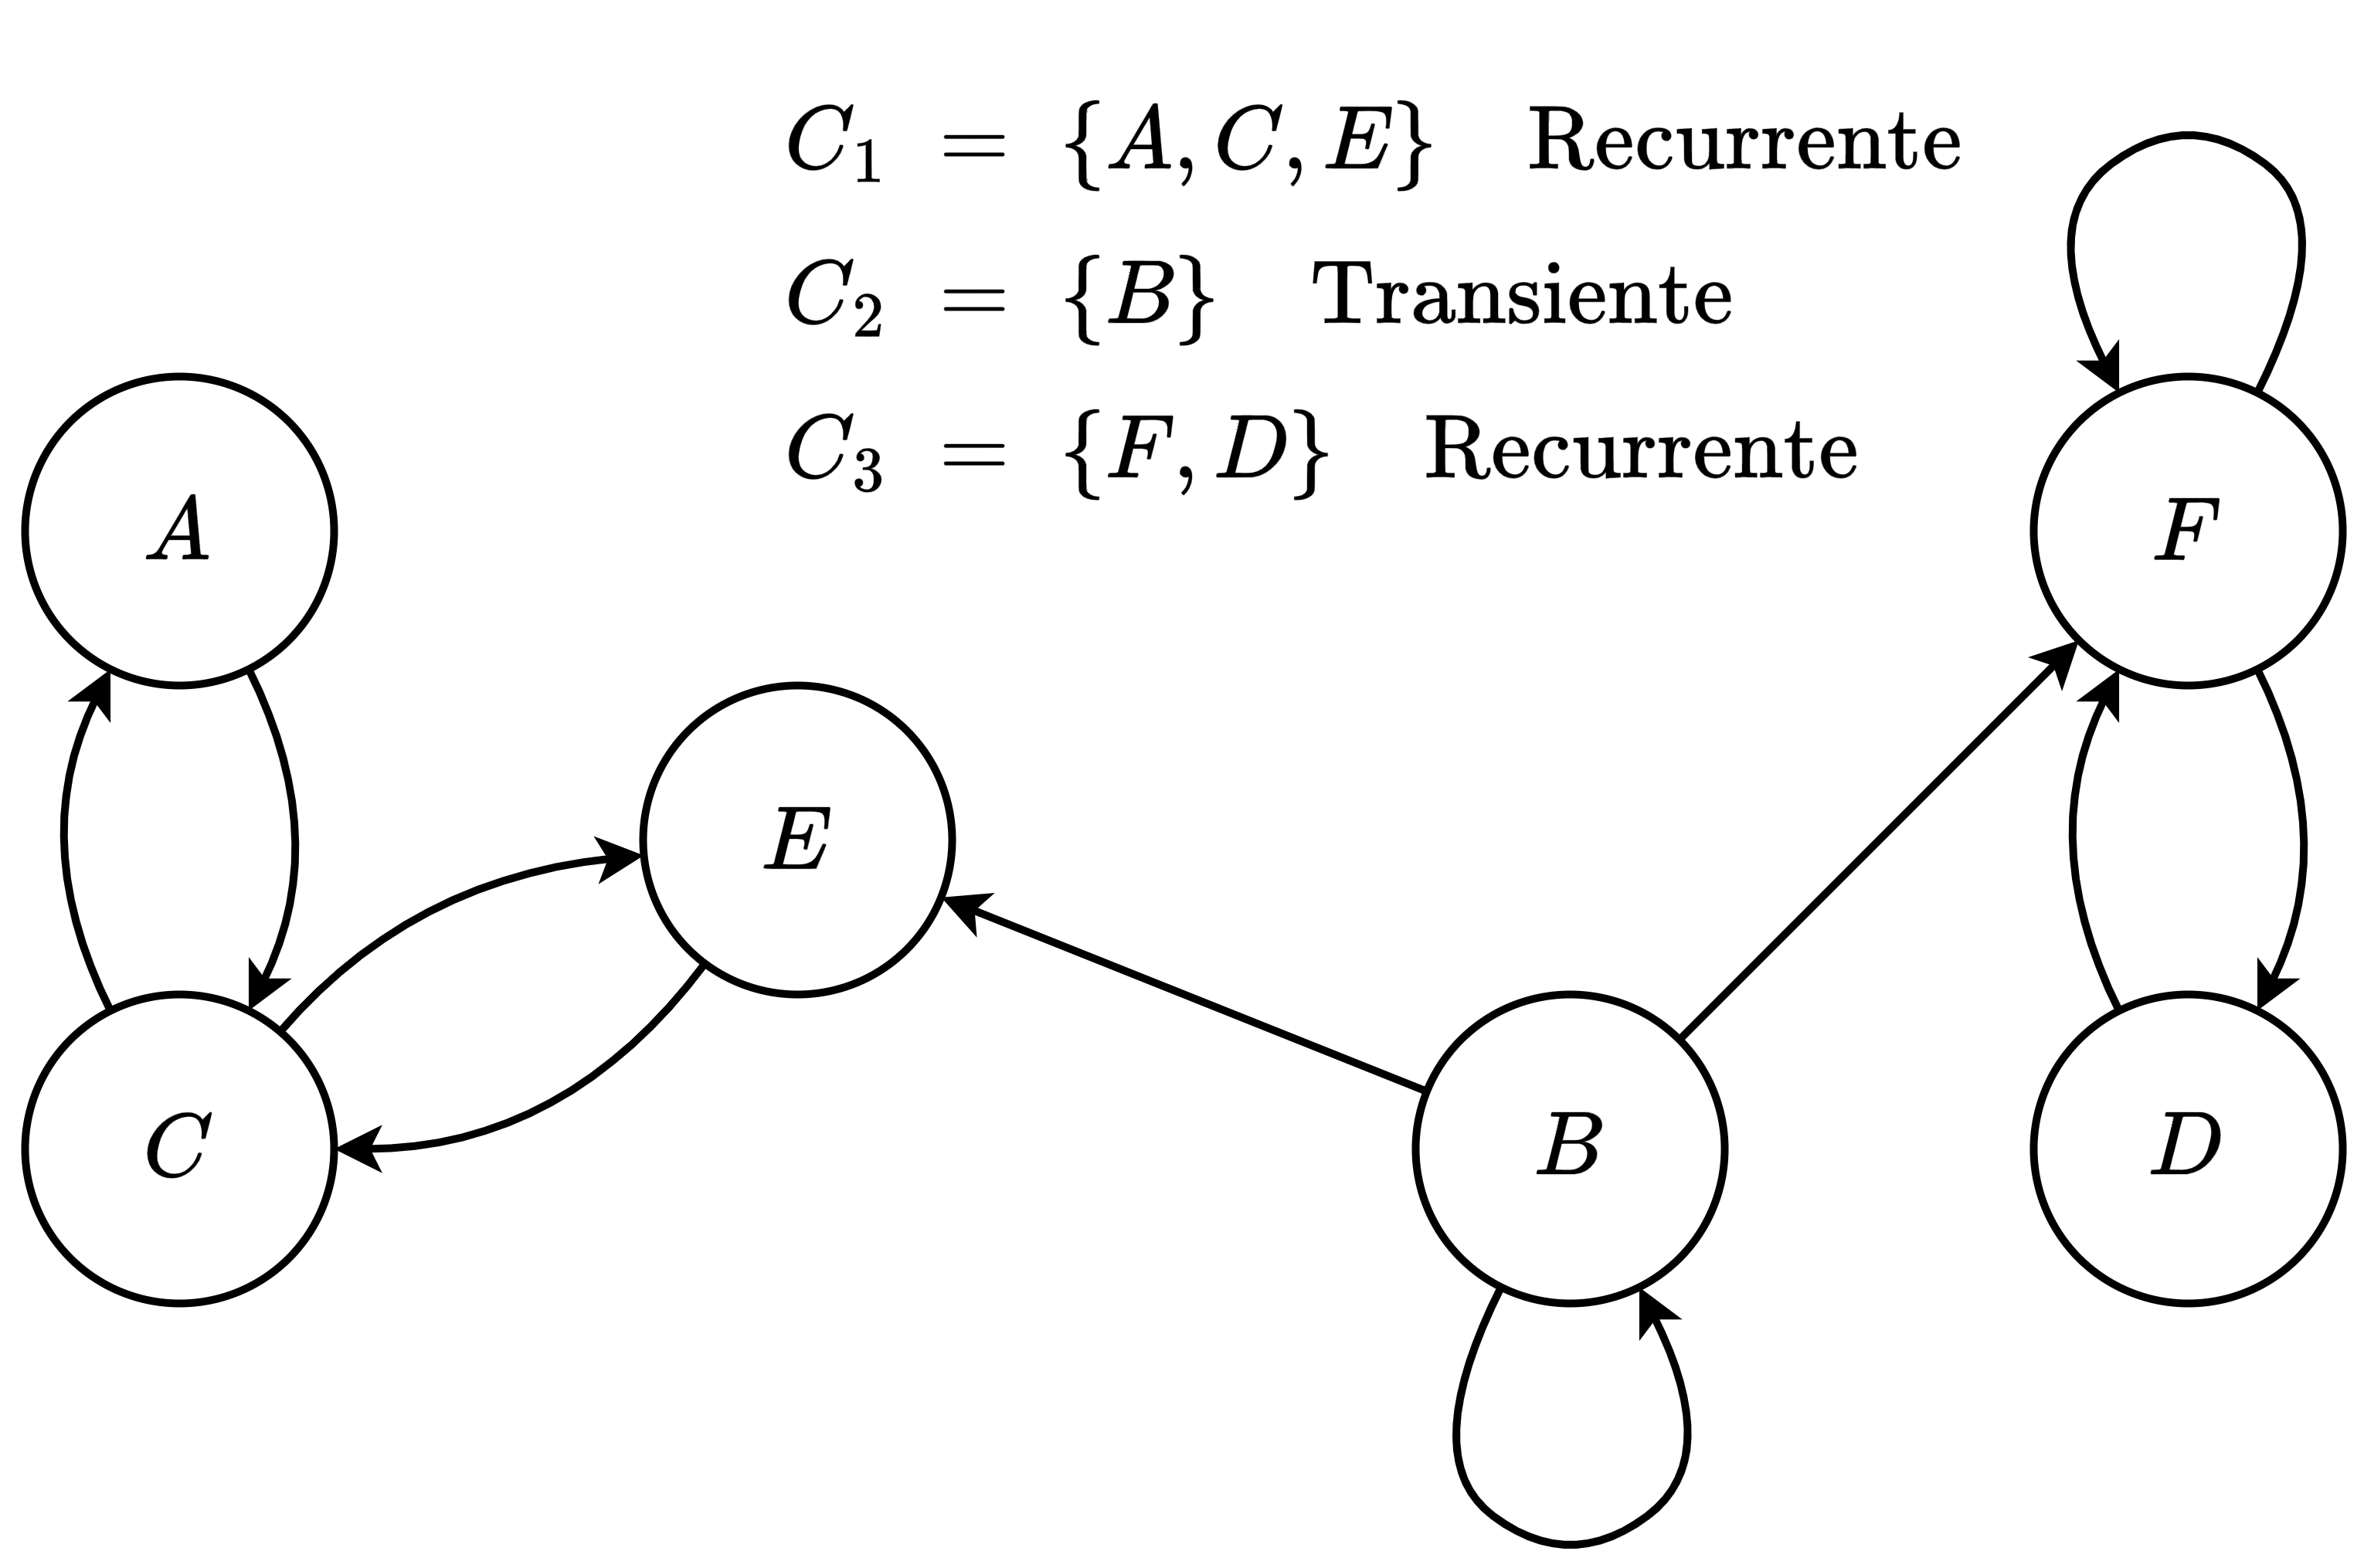
\includegraphics[width=0.6\textwidth]{diagram/DTEEC.png}
\end{figure}
\subsection{Erg\'odica}
Una cadena se dice erg\'odica si es irreducible, recurrente y aperi\'odica.
\begin{itemize}
    \item Para este tipo de cadena podemos determinar el vector pi.
    \begin{equation*}
        \scalebox{1.5}{$\vec{\pi}$} = \left(\pi_1, \pi_2, ..., \pi_k\right) \quad \sum{\pi_i} = 1
    \end{equation*}
\end{itemize}
\subsubsection{Distribución de estado o de largo plazo}
\begin{minipage}{0.45\textwidth}
    \begin{figure}[H]
        \centering
        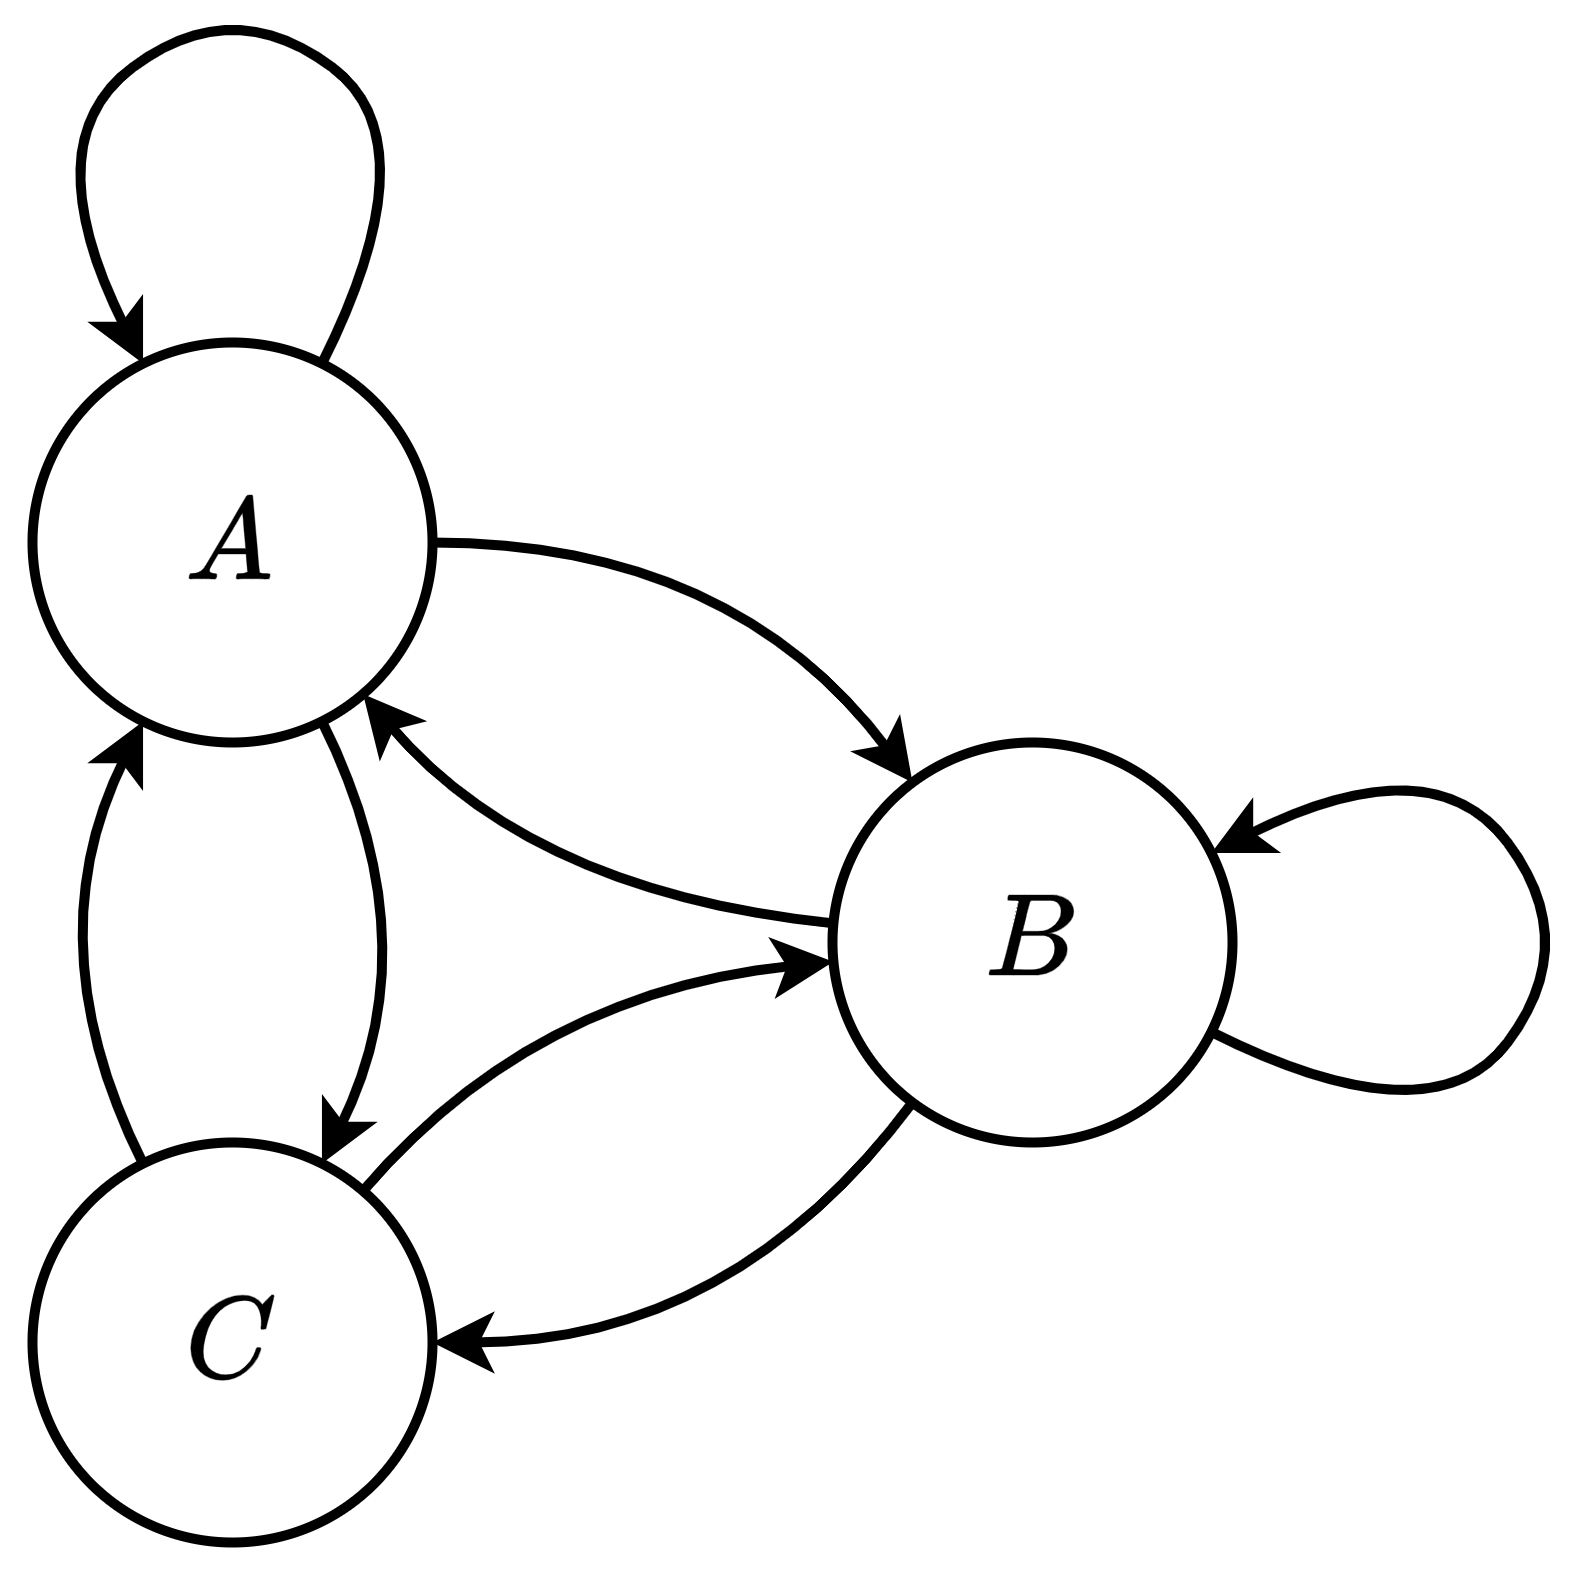
\includegraphics[width=0.7\textwidth]{diagram/DTEDist.png}
    \end{figure}
\end{minipage}
\hfill
\begin{minipage}[ht]{0.45\textwidth}
    \begin{equation*}
        A, A, B, B, C, A, A, C, A, B
    \end{equation*}
    \begin{equation*}
        \scalebox{1.5}{$\pi$}_A = \frac{5}{10} \qquad \scalebox{1.5}{$\pi$}_B = \frac{3}{10} \qquad \scalebox{1.5}{$\pi$}_C = \frac{2}{10}
    \end{equation*}
\end{minipage}

\subsection{Teorema 1}
Cuando $P$ es la matriz de transición en una etapa de una cadena ergódica.
\begin{equation*}
    \lim_{n \to \infty}{P^n} = \scalebox{1.5}{$\vec{\pi}$}
\end{equation*}

\subsection{Teorema 2}
\begin{equation*}
    \scalebox{1.5}{$\vec{\pi}$} = \scalebox{1.5}{$\vec{\pi}$} \cdot P \qquad \sum{\pi_i} = 1
\end{equation*}

\subsection{Problema 4}
¿Que porcentaje de mercado captura cada competidor en el largo plazo?
\begin{figure}[H]
    \centering
    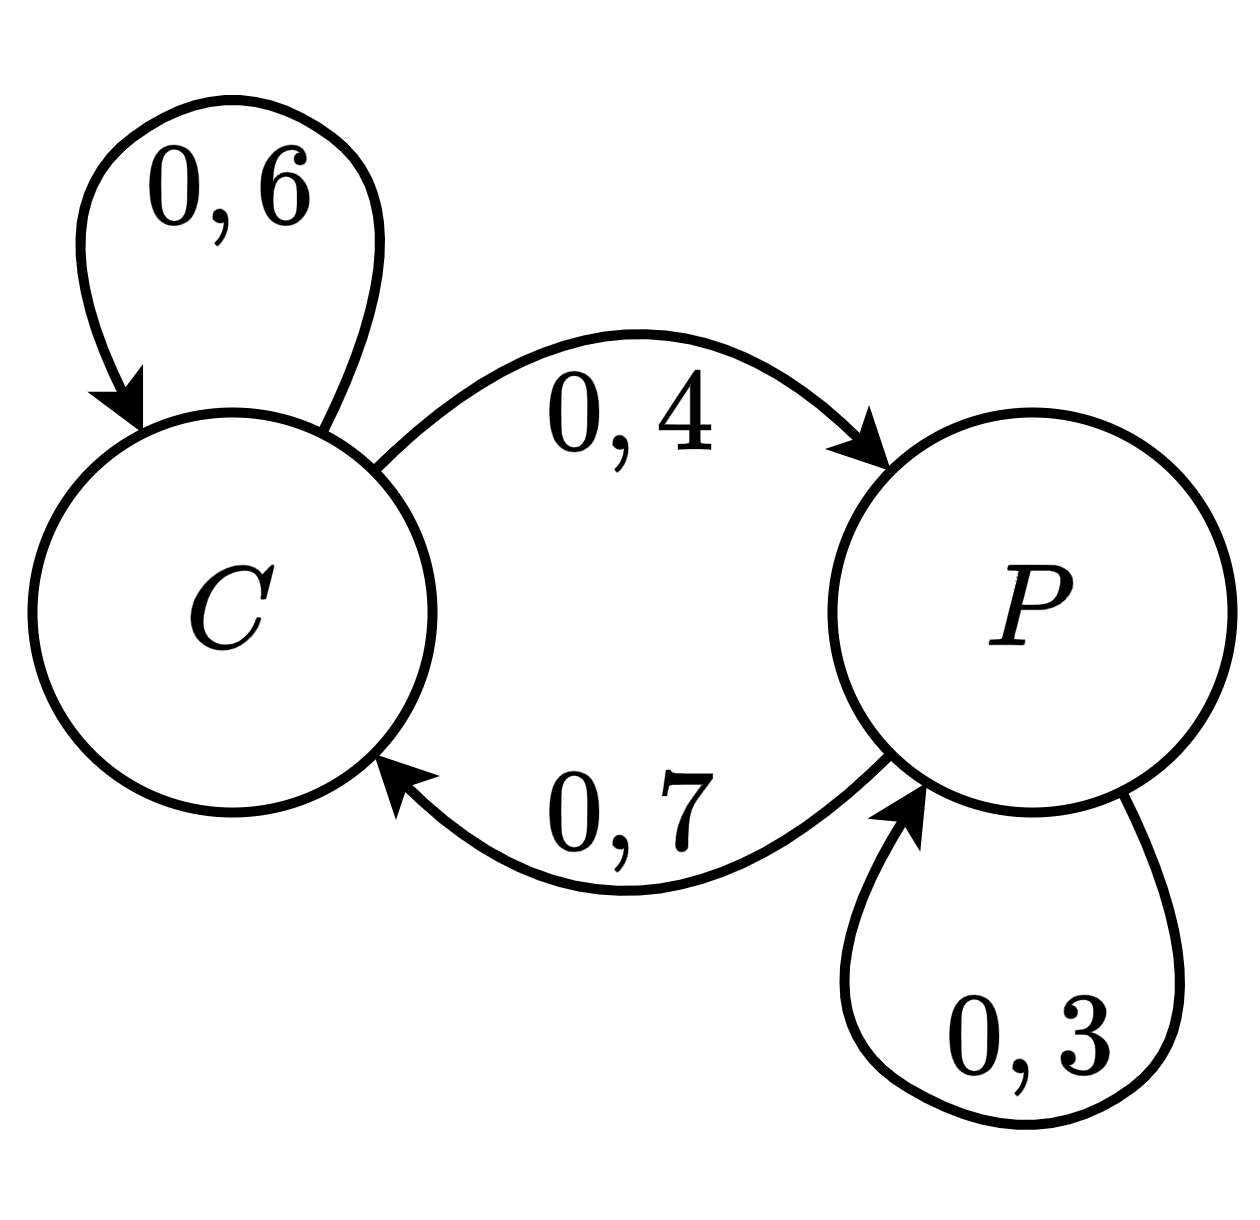
\includegraphics[width=0.3\textwidth]{diagram/DTE4.png}
\end{figure}
Para encontrar el porcentaje de mercado capturado por cada competidor, se debe calcuar la distribución de largo plazo.
\begin{equation*}
    \scalebox{1.5}{$\vec{\pi}$} = \left(\pi_1 \; \pi_2\right) \cdot \left(\begin{matrix}
        0,6 & 0,4 \\
        0,7 & 0,3
    \end{matrix}\right)
\end{equation*}
\begin{eqnarray*}
    \pi_1 &= 0,6 \pi_1 + 0,7 \pi_2 \\
    \pi_2 &= 0,4 \pi_1 + 0,3 \pi_2
\end{eqnarray*}
Igualamos las ecuaciones y despejamos.
\begin{eqnarray*}
    -0.4 \pi_1 + 0.7 \pi_2 &= 0 \\
    0.4 \pi_1 - 0.7 \pi_2 &= 0
\end{eqnarray*}
Para encontrar, valores distintos a la solucion nula se remplaza cualquiera de las ecuaciones por $\sum \pi_i = 1$.
\begin{eqnarray*}
    0.4 \pi_1 - 0.7 \pi_2 &= 0 \\
    \pi_1 + \pi_2 &= 1
\end{eqnarray*}

Para $\pi_1$.
\begin{align*}
    0.4 \pi_1 - 0.7 \pi_2 &= 0 \\
    0.7 \pi_1 + 0.7 \pi_2 &= 0.7 \\
    \\
    1.1 \pi_1 &= 0.7 \\
    \pi_1 &= \frac{0.7}{1.1} = 0.64
\end{align*}

Para $\pi_2$.
\begin{align*}
    \pi_1 + \pi_2 &= 1 \\
    0.64 + \pi_2 &= 1 \\
    \pi_2 &= 1 - 0.64 = 0.36
\end{align*}
Asi, los porcentajes de mercado capturados por cada competidor son:
\begin{eqnarray*}
    \pi_1 &= 0,64 = 64\% \\
    \pi_2 &= 0,36 = 36\%
\end{eqnarray*}

\newpage
\section{Listado cadenas de markov}
\begin{enumerate}
    \item Calcular las participaciones en el mercado que a largo plazo alcanzarán las compañias R, S y T, si el comportamiento de los consumidores corresponde a una cadena de Markov con las probabilidades de cambio que se muestran en la tabla.
    \begin{center}
        \begin{tabular}{g|c|c|c|c|}
            \rowcolor{Celeste!50}
            \cellcolor{white} & \textbf{R} & \textbf{S} & \textbf{T} \\
            \hline
            \textbf{R} & 0,6 & 0,1 & 0,3 \\
            \hline
            \textbf{S} & 0,5 & 0,4 & 0,1 \\
            \hline
            \textbf{T} & 0,2 & 0,1 & 0,7 \\
            \hline
        \end{tabular}
    \end{center}
    Para encontrar el porcentaje de mercado capturado por cada competidor, se debe calcuar la distribución de largo plazo.
    \begin{equation*}
        \scalebox{1.5}{$\vec{\pi}$} = \left(\pi_1 \; \pi_2 \; \pi_3\right) \cdot \left(\begin{matrix}
            0,6 & 0,1 & 0,3 \\
            0,5 & 0,4 & 0,1 \\
            0,2 & 0,1 & 0,7
        \end{matrix}\right)
    \end{equation*}

    \begin{eqnarray*}
        \pi_1 &= 0,6 \pi_1 + 0,5 \pi_2 + 0,2 \pi_3 \\
        \pi_2 &= 0,1 \pi_1 + 0,4 \pi_2 + 0,1 \pi_3 \\
        \pi_3 &= 0,3 \pi_1 + 0,1 \pi_2 + 0,7 \pi_3
    \end{eqnarray*}

    Igualamos las ecuaciones y despejamos.
    \begin{eqnarray*}
        -0.4 \pi_1 + 0.5 \pi_2 + 0.2 \pi_3 &= 0 \\
        0.1 \pi_1 - 0.6 \pi_2 + 0.1 \pi_3 &= 0 \\
        0.3 \pi_1 + 0.1 \pi_2 - 0.3 \pi_3 &= 0
    \end{eqnarray*}

    Para encontrar una solucion distinta a la nula, se remplaza cualquiera de las ecuaciones por $\sum \pi_i = 1$.
    \begin{eqnarray*}
        -0.4 \pi_1 + 0.5 \pi_2 + 0.2 \pi_3 &= 0 \\
        0.1 \pi_1 - 0.6 \pi_2 + 0.1 \pi_3 &= 0 \\
        \pi_1 + \pi_2 + \pi_3 &= 1
    \end{eqnarray*}

    Se resuelve el sistema de ecuaciones.
    \begin{eqnarray*}
        \pi_1 &= 0,41 \\
        \pi_2 &= 0,14 \\
        \pi_3 &= 0,45
    \end{eqnarray*}

    Asi, los porcentajes de mercado capturados por cada competidor son:
    \begin{itemize}
        \item Para la compa\~nia R: 41\%
        \item Para la compa\~nia S: 14\%
        \item Para la compa\~nia T: 45\%
    \end{itemize}

    \newpage
    \item En una población de 10.000 habitantes, 5.000 no fuman, 2.500 fuman uno o menos de un paquete diario y 2.500 fuman más de un paquete diario. En un mes hay un 5\% de probabilidad de que un no fumador comience a fumar un paquete diario o menos, y un 2\% de que un no fumador pase a fumar más de un paquete diario. Para los que fuman un paquete o menos, hay un 10\% de probabilidad de que dejen el tabaco, y un 10\% de que pasen a fumar más de un paquete diario. Entre los que fuman más de un paquete, hay un 5\% de probabilidad de que dejen el tabaco y un 10\% de que pasen a fumar un paquete o menos. ¿Cuántos individuos habrán de cada clase el próximo mes?
    
    \begin{center}
        \begin{tabular}{g|c|c|c|}
            \rowcolor{Celeste!50}
            \cellcolor{white} & \textbf{No fumador} & \textbf{Fuma 1 o menos} & \textbf{Fuma más de 1} \\
            \hline
            \textbf{No fumador} & 0,93 & 0,05 & 0,02 \\
            \hline
            \textbf{Fuma 1 o menos} & 0,1 & 0,8 & 0,1 \\
            \hline
            \textbf{Fuma más de 1} & 0,05 & 0,1 & 0,85 \\
            \hline
        \end{tabular}
    \end{center}

    \begin{itemize}
        \item $\pi_1$ : 5.000 de 10.000 son no fumadores.
        \item $\pi_2$ : 2.500 de 10.000 fuman 1 o menos paquete diario.
        \item $\pi_3$ : 2.500 de 10.000 fuman más de 1 paquete diario.
    \end{itemize}
    Sabemos que la distribución inicial es:
    \begin{align*}
        \scalebox{1.5}{$\vec{\pi}$}_{(0)} &= \left(0.5 \; 0.25 \; 0.25\right)
    \end{align*}

    Necesitamos la distribución de largo plazo del próximo mes.
    \begin{align*}
        \scalebox{1.5}{$\vec{\pi}$}_{(1)} &= \left(0.5 \; 0.25 \; 0.25\right) \cdot \left(\begin{matrix}
            0,93 & 0,05 & 0,02 \\
            0,1 & 0,8 & 0,1 \\
            0,05 & 0,1 & 0,85
        \end{matrix}\right)^1 \\
        &= \left(0.5025 \; 0.25 \; 0.2475\right)
    \end{align*}

    Asi, el próximo mes habrán:
    \begin{itemize}
        \item 5.025 no fumadores.
        \item 2.500 fumadores de 1 o menos paquete diario.
        \item 2.475 fumadores de más de 1 paquete diario.
    \end{itemize}

    \newpage
    \item Clasificar los estados de las cadenas de Markov con las siguientes matrices de transición:
    \begin{enumerate}
        \item \textbf{Matriz de transición 3}
        \begin{align*}
            P &= \left(\begin{matrix}
                0.5 & 0.5 & 0 & 0 & 0 \\
                0.5 & 0.5 & 0 & 0 & 0 \\
                0 & 0 & 0.5 & 0.5 & 0 \\
                0 & 0 & 0.5 & 0.5 & 0 \\
                0.25 & 0.25 & 0 & 0 & 0.5
            \end{matrix}\right)
        \end{align*}

        \begin{center}
            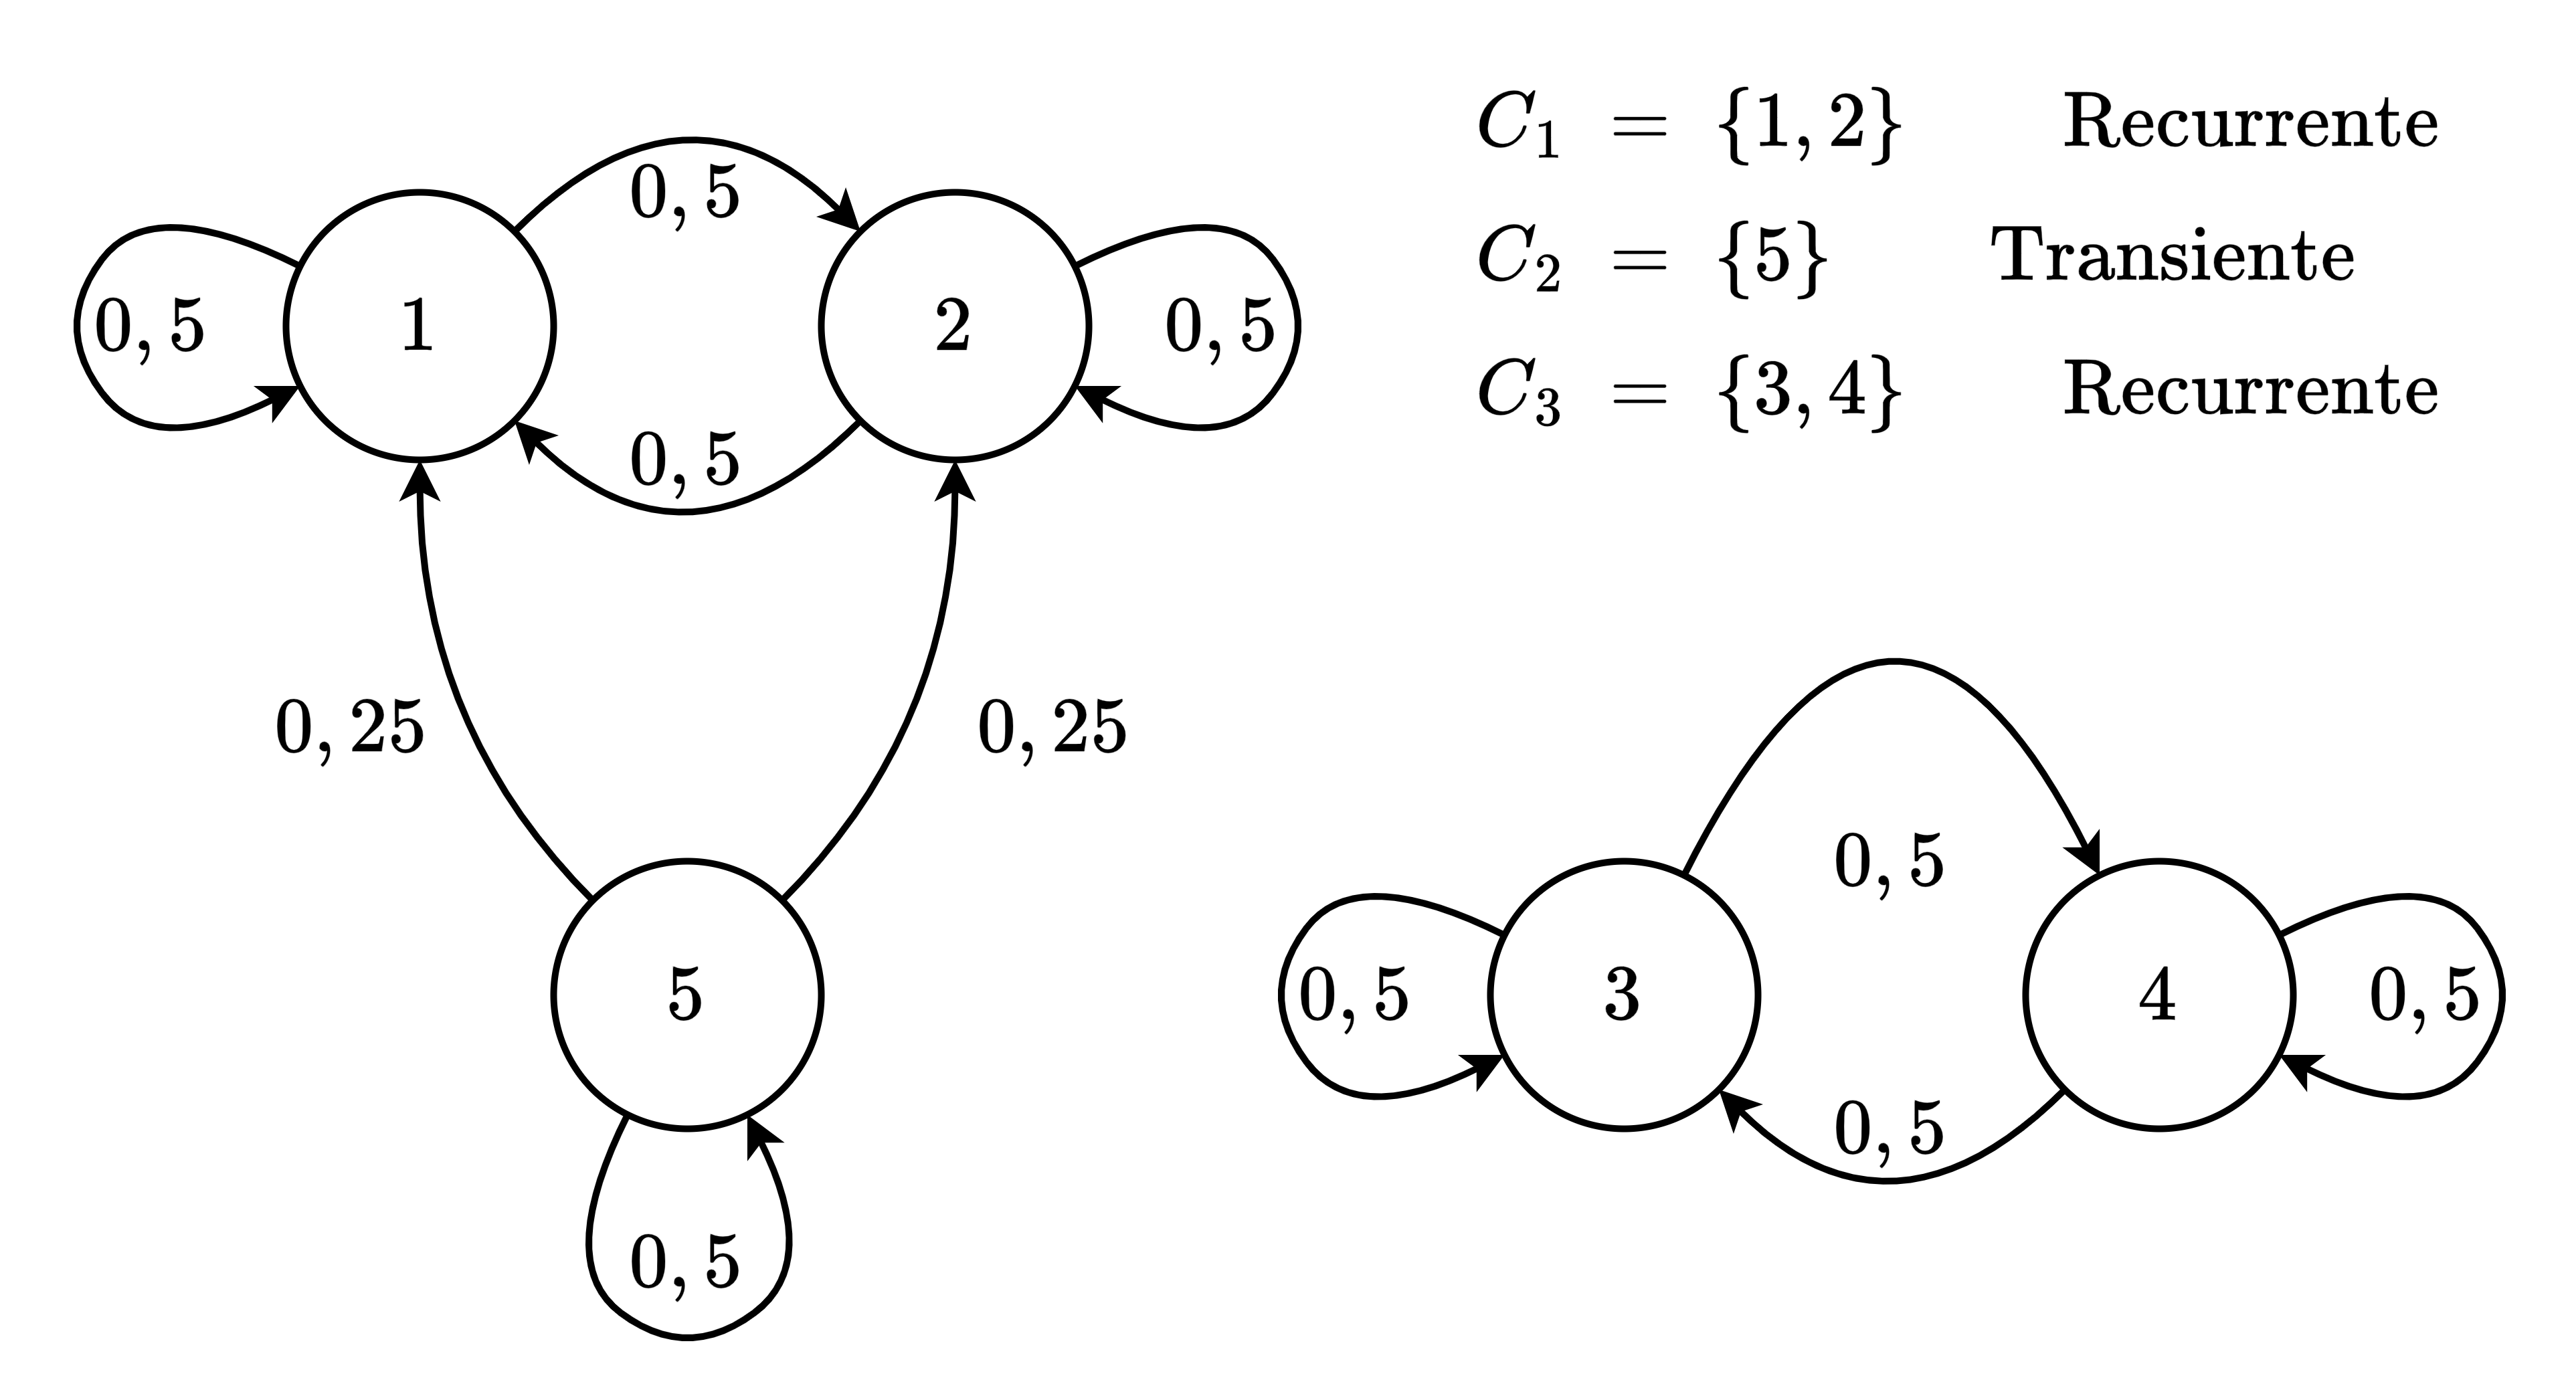
\includegraphics[width=0.85\textwidth]{diagram/P-3.png}
        \end{center}

        Por lo tanto, la matriz de transición 3 es \textbf{reductible}.
    \end{enumerate}
\end{enumerate}
\end{document}
